\section{Results}\label{sec:results}

\subsection{Task Difficulty: Trivial Baseline Analysis}

We first establish the inherent difficulty of the three-class toolpath discrimination task. Table~\ref{tab:trivial_baselines} reports classification accuracy using only trivial metadata features (no sensor data).

\begin{table}[H]
\caption{Classification accuracy using trivial (non-sensor) features only, with the RF classifier and 5-fold CV. These features are derived from machine state columns, not from the IMU or electrical sensor data.}\label{tab:trivial_baselines}
\centering
\begin{tabular}{lcc}
\toprule
\textbf{Feature Set} & \textbf{Accuracy (\%)} & \textbf{Features} \\
\midrule
G-code line range (min, max, range, nunique)  & $100.0 \pm 0.0$ & 4 \\
Mean axis position (X, Y, Z)                  & $98.0 \pm 4.0$  & 3 \\
Row count (program duration)                  & $98.0 \pm 4.0$  & 1 \\
All trivial metadata                          & $100.0 \pm 0.0$ & 22 \\
Mean feed rate                                & $90.4 \pm 8.6$  & 2 \\
Random noise                                  & $35.3 \pm 7.8$  & 10 \\
\bottomrule
\end{tabular}
\end{table}

The trivial baselines reveal that the three toolpath types are inherently separable from program metadata alone. The G-code line range achieves 100\% accuracy because the three toolpath programs have different line counts (985, 111, and 193 lines for adaptive, face, and pocket, respectively). Mean axis position achieves 98\% because each program traverses a different region of the machine's workspace. This contextualizes all subsequent results. Perfect classification of these three toolpath types does not \textit{per se} validate the sensor-based methodology. Instead, the value of the sensor-based approach lies in its potential applicability to scenarios where metadata is unavailable or insufficient, such as cross-machine transfer, within-toolpath-type parameter discrimination, or anomaly detection.

\subsection{Sensor-Based Classification Performance}

Table~\ref{tab:main_results} reports the sensor-based classification accuracy using temporal-binned features ($B = 20$ bins, 1{,}540 features per run).

\begin{table}[H]
\caption{Sensor-based classification accuracy (\%) for each isolation method and classifier, without PCA. Results are mean $\pm$ standard deviation across 5-fold stratified CV.}\label{tab:main_results}
\centering
\begin{tabular}{lccc}
\toprule
\textbf{Isolation Method} & \textbf{RF} & \textbf{SVM} & \textbf{MLP} \\
\midrule
Raw          & $100.0 \pm 0.0$ & $90.0 \pm 7.1$ & $86.0 \pm 11.4$ \\
Subtracted   & $100.0 \pm 0.0$ & $94.0 \pm 8.9$ & $94.2 \pm 8.9$ \\
Ratio        & $100.0 \pm 0.0$ & $94.0 \pm 8.9$ & $96.0 \pm 5.5$ \\
Z-score      & $100.0 \pm 0.0$ & $94.0 \pm 5.5$ & $94.0 \pm 5.5$ \\
\bottomrule
\end{tabular}
\end{table}

RF achieves 100\% accuracy across all four isolation methods. While this result is consistent with the trivial baseline analysis (the task is inherently easy), the sensor features achieve it without access to program metadata. The isolation methods improve accuracy for SVM (+4--8 pp over raw) and MLP (+8--10 pp), suggesting that air-cut referencing removes noise or machine-specific variation that these classifiers are sensitive to.

\subsection{Repeated Cross-Validation: Robustness Analysis}

Standard 5-fold CV provides only 5 accuracy estimates, insufficient for reliable variance estimation. Table~\ref{tab:repeated_cv} reports results from 20 repeats $\times$ 5-fold CV (100 total evaluations per configuration).

\begin{table}[H]
\caption{Repeated CV accuracy (20$\times$5-fold = 100 evaluations). The ``Min'' column reveals the worst-case fold accuracy, which differentiates methods that standard mean$\pm$std cannot.}\label{tab:repeated_cv}
\centering
\begin{tabular}{llcccc}
\toprule
\textbf{Method} & \textbf{Clf} & \textbf{Mean} & \textbf{Std} & \textbf{Min} & \textbf{Max} \\
\midrule
Raw        & RF  & 98.9 & 3.1 & 90.0 & 100.0 \\
Subtracted & RF  & 100.0 & 0.0 & 100.0 & 100.0 \\
Ratio      & RF  & 100.0 & 0.0 & 100.0 & 100.0 \\
Z-score    & RF  & 100.0 & 0.0 & 100.0 & 100.0 \\
\midrule
Raw        & SVM & 88.8 & 9.3 & 60.0 & 100.0 \\
Subtracted & SVM & 92.4 & 8.6 & 60.0 & 100.0 \\
Ratio      & SVM & 92.6 & 8.4 & 60.0 & 100.0 \\
Z-score    & SVM & 91.8 & 9.4 & 50.0 & 100.0 \\
\midrule
Ratio      & MLP & 96.5 & 5.6 & 80.0 & 100.0 \\
Z-score    & MLP & 95.0 & 6.7 & 70.0 & 100.0 \\
\bottomrule
\end{tabular}
\end{table}

In the repeated CV, \textbf{raw RF occasionally misclassifies} (minimum fold accuracy 90\%), while subtracted, ratio, and z-score RF maintain perfect accuracy across all 100 evaluations; this difference is invisible in the standard 5-fold results. Per-sample analysis across all 20 repeats identifies one specific run, pocket150025\_001, that raw RF misclassifies in 55\% of evaluations, while all three referenced methods classify it correctly in 100\% of evaluations.

\subsection{Statistical Significance Analysis}

We apply several complementary significance tests to the 100 fold-level accuracy values from the repeated CV.

\textbf{Friedman test.} A Friedman non-parametric ANOVA across the four isolation methods (using RF) yields $\chi^2 = 33.0$, $p < 10^{-6}$, confirming that the methods do not perform equally. Post-hoc pairwise Wilcoxon signed-rank tests with Bonferroni correction show that raw is significantly different from each referenced method ($p_{\mathrm{Bonf}} = 0.011$ for raw vs.\ subtracted, ratio, and z-score), while the three referenced methods are statistically indistinguishable ($p = 1.0$). A separate Friedman test across classifiers (RF vs.\ SVM vs.\ MLP, using subtracted features) yields $\chi^2 = 87.3$, $p < 10^{-6}$, confirming that classifier choice significantly affects accuracy.

\textbf{Two-way ANOVA.} A two-way analysis of variance (isolation method $\times$ classifier) reveals that both main effects are significant: method ($F = 4.18$, $p = 0.006$, $\eta^2 = 0.04$) and classifier ($F = 31.2$, $p < 10^{-6}$, $\eta^2 = 0.17$). The classifier effect accounts for approximately 4$\times$ more variance than the isolation method, indicating that the choice of learning algorithm dominates the choice of signal referencing strategy for this classification task.

\textbf{Bootstrap confidence intervals.} Figure~\ref{fig:bootstrap_ci} shows bootstrap 95\% confidence intervals (1{,}000 bootstrap samples) for the RF accuracy of each isolation method. The raw method's CI $[0.982, 0.994]$ does not overlap with the referenced methods' CI $[1.000, 1.000]$, confirming the robustness difference at the 95\% confidence level.

\begin{figure}[H]
    \centering
    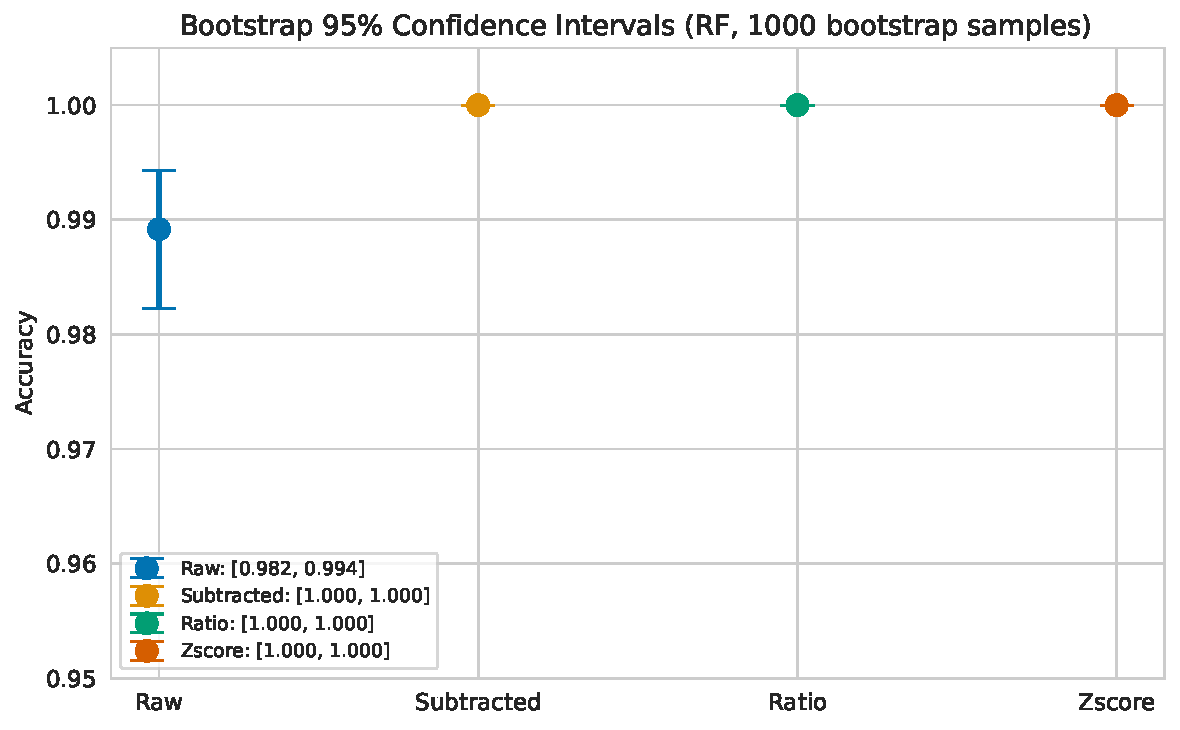
\includegraphics[width=0.7\textwidth]{figures/fig12_bootstrap_ci.pdf}
    \caption{Bootstrap 95\% confidence intervals for RF classification accuracy by isolation method. The raw method's interval $[0.982, 0.994]$ does not overlap with the referenced methods $[1.000, 1.000]$.}
    \label{fig:bootstrap_ci}
\end{figure}

\textbf{Effect size.} Cohen's $d$ for raw vs.\ each referenced method is $d = 0.49$. However, Cohen's $d$ assumes approximately normal distributions away from boundaries, which is violated here (referenced methods have zero variance at the 100\% ceiling). A more appropriate non-parametric measure is Cliff's delta, which quantifies the probability that a randomly chosen fold from the referenced method outperforms one from the raw method. With 100 raw-method folds and 100 referenced-method folds, Cliff's $\delta = 0.022$ (the proportion of pairs where raw $<$ referenced minus the proportion where raw $>$ referenced), because raw achieves 100\% in most folds but fails in a small fraction. The degenerate bootstrap CI $[1.000, 1.000]$ for referenced methods reflects a performance ceiling rather than precise estimation.

\textbf{Caveats on higher-order statistics.} The temporal bins contain 6--39 timesteps each (depending on run length and bin count). Computing skewness and kurtosis from such small samples yields unreliable 3rd and 4th moment estimates. The feature statistic ablation (Section~\ref{sec:ablation}) shows that mean + RMS alone (2 statistics, no higher-order moments) achieves 98\% accuracy, confirming that the classification does not depend critically on these unreliable estimators.

\textbf{ANOVA caveat.} The two-way ANOVA reported above assumes normality and independence of fold-level accuracy scores. With accuracy bounded at $[0, 1]$ and strong ceiling effects, these assumptions are violated. The Friedman test (non-parametric) provides the more reliable significance assessment; the ANOVA $\eta^2$ values should be interpreted as approximate effect size indicators rather than exact variance decompositions.

\subsection{Comparison Against Time-Series Methods}

To contextualize our temporal-binning feature extraction against modern time-series classification approaches, Table~\ref{tab:rocket} compares against ROCKET-style random convolutional features~\cite{dempster2020rocket}.

\begin{table}[H]
\caption{Comparison of feature extraction approaches. ROCKET uses 1{,}000 random convolutional kernels applied directly to the raw sensor time series.}\label{tab:rocket}
\centering
\begin{tabular}{lcc}
\toprule
\textbf{Method} & \textbf{Accuracy (\%)} & \textbf{Features} \\
\midrule
Temporal binning + RF (ours)           & $100.0 \pm 0.0$ & 1{,}540 \\
ROCKET + RF                            & $100.0 \pm 0.0$ & 2{,}000 \\
ROCKET + Ridge                         & $98.0 \pm 4.0$  & 2{,}000 \\
Raw downsampled (50 steps) + RF        & $98.0 \pm 4.0$  & 5{,}500 \\
\bottomrule
\end{tabular}
\end{table}

ROCKET with RF matches our approach at 100\% accuracy, while ROCKET with Ridge achieves 98\%. This confirms that the classification task is solvable by multiple feature extraction strategies, consistent with the trivial baseline findings. However, our temporal binning approach offers the advantage of interpretable temporal fingerprints (Section~\ref{sec:fingerprints}) and a natural framework for air-cut referencing that ROCKET does not provide.

\subsection{PCA Visualization}

Figure~\ref{fig:pca_scatter} shows the first two principal components for each isolation method.

\begin{figure}[H]
    \centering
    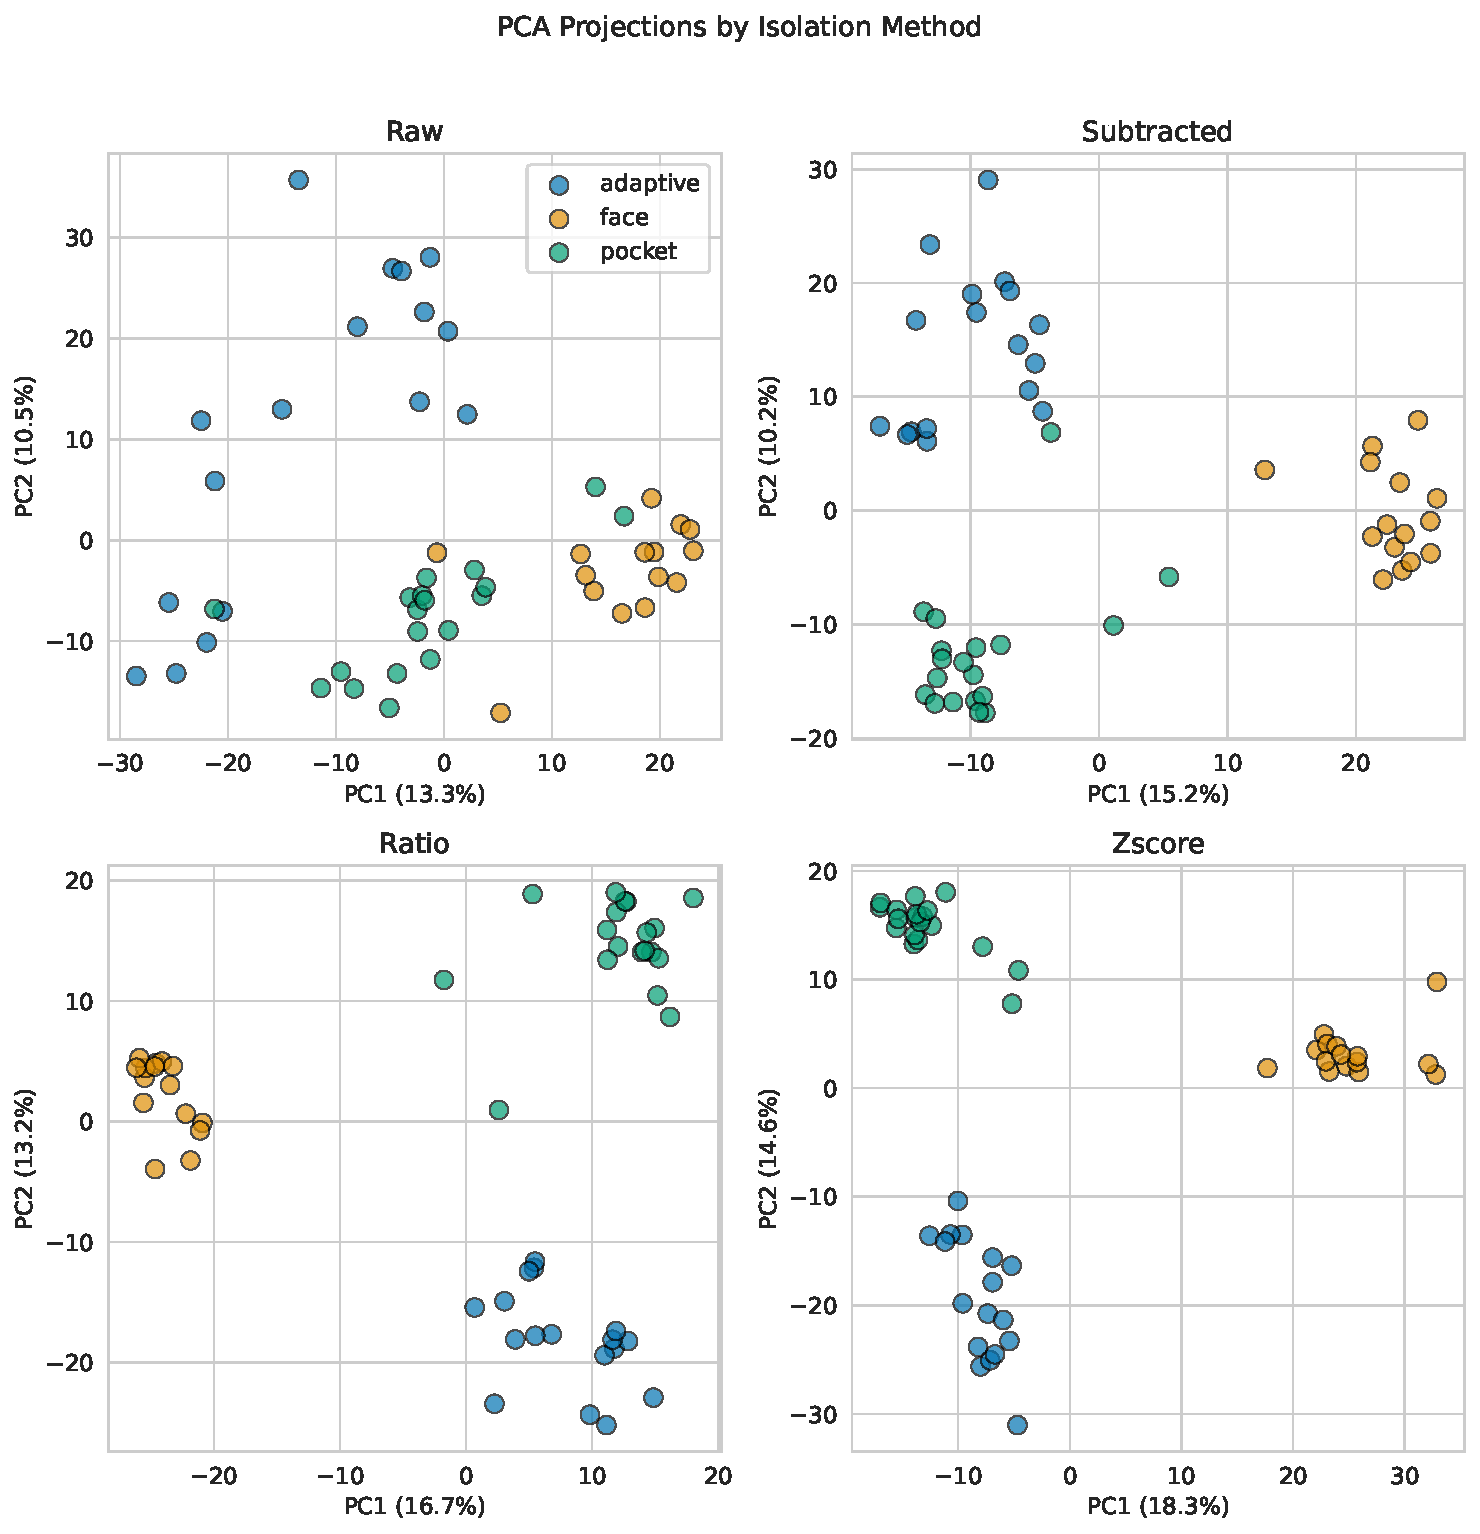
\includegraphics[width=0.85\textwidth]{figures/fig2_pca_scatter.pdf}
    \caption{PCA projections for each isolation method. Each point represents one active-cutting run (51 total), colored by toolpath type.}
    \label{fig:pca_scatter}
\end{figure}

All four methods produce visible cluster separation. The z-score method shows the tightest within-class clusters, consistent with its strong performance across classifiers.

\subsection{Feature Importance and Physical Interpretation}\label{sec:physics}

Figure~\ref{fig:importance} shows the top 20 features by RF Gini importance.

\begin{figure}[H]
    \centering
    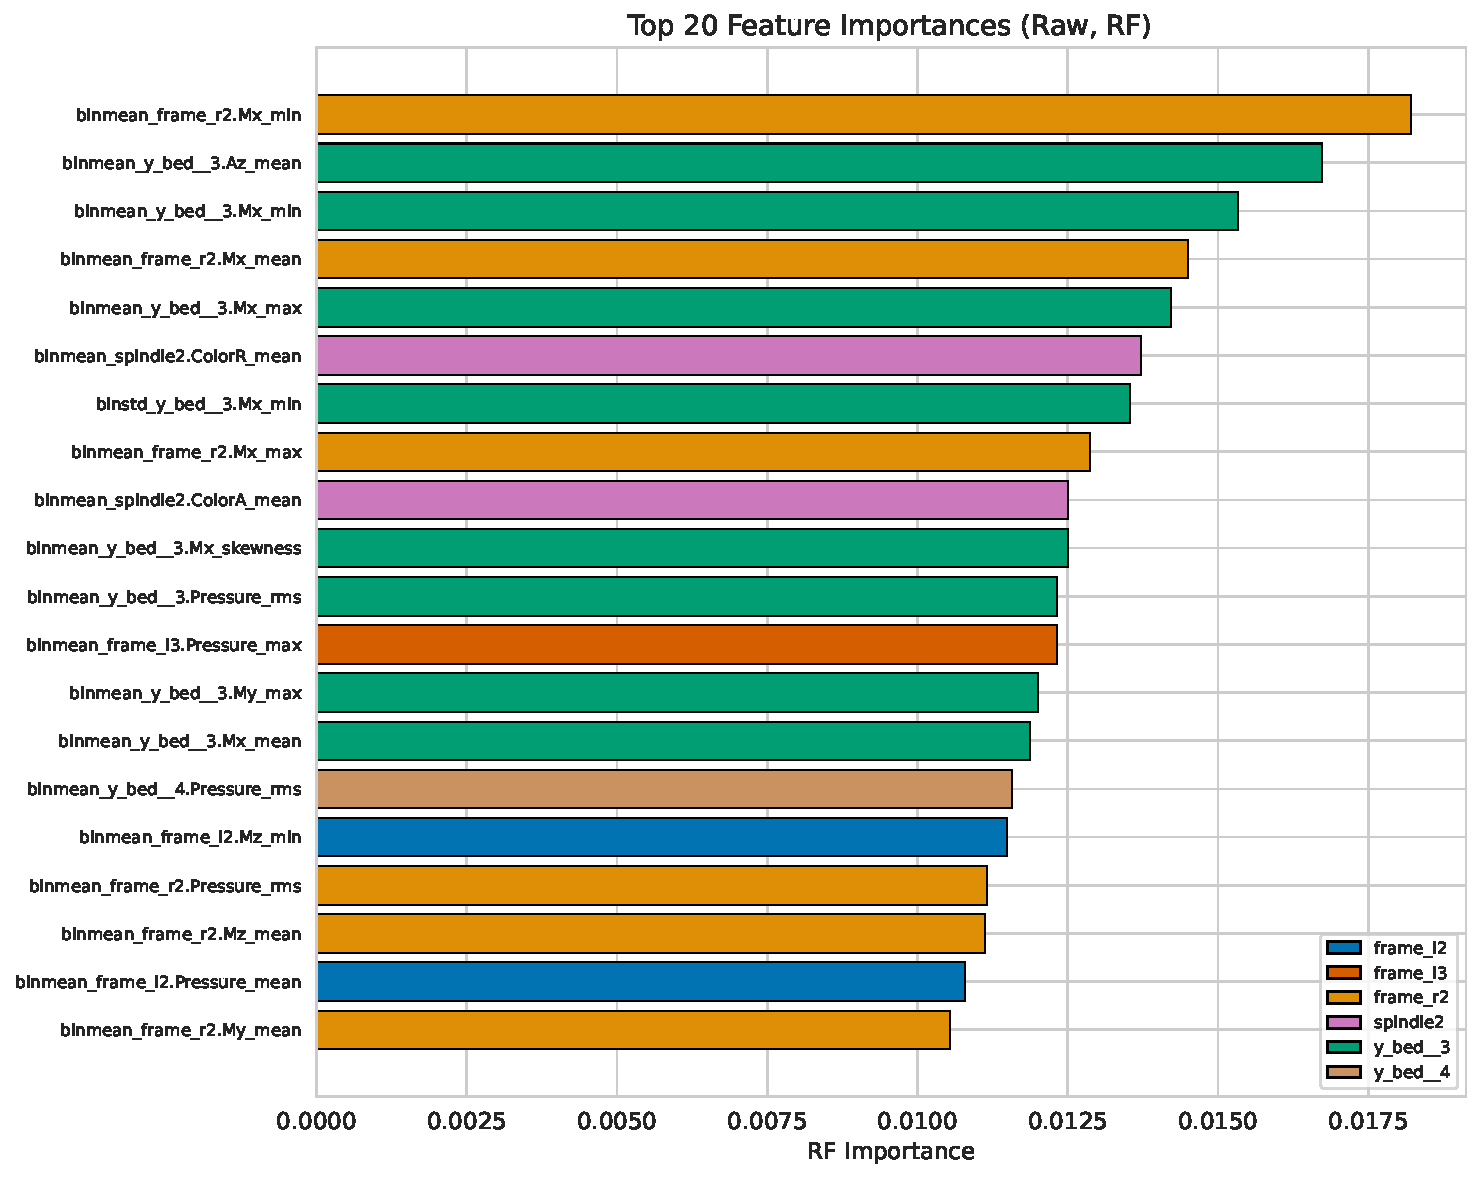
\includegraphics[width=0.85\textwidth]{figures/fig5_importance.pdf}
    \caption{Top 20 features by RF importance, colored by sensor module.}
    \label{fig:importance}
\end{figure}

Among the top 50 features, magnetometer channels dominate (24 features, 26.5\% of total importance), followed by environmental channels (pressure, temperature, proximity; 14 features, 13.4\%) and color sensors (6 features, 6.0\%). Accelerometer and gyroscope channels, which one might expect to dominate based on cutting force mechanics, account for only 2 of the top 50 features. Among sensor modules, y\_bed\_\_3 (bed-mounted, 17 features) and frame\_r2 (frame right, 13 features) contribute most.

To understand \emph{why} these channels dominate, Figure~\ref{fig:physical_interpretation} plots four physically distinct sensor channels across the three toolpath types.

\begin{figure}[H]
    \centering
    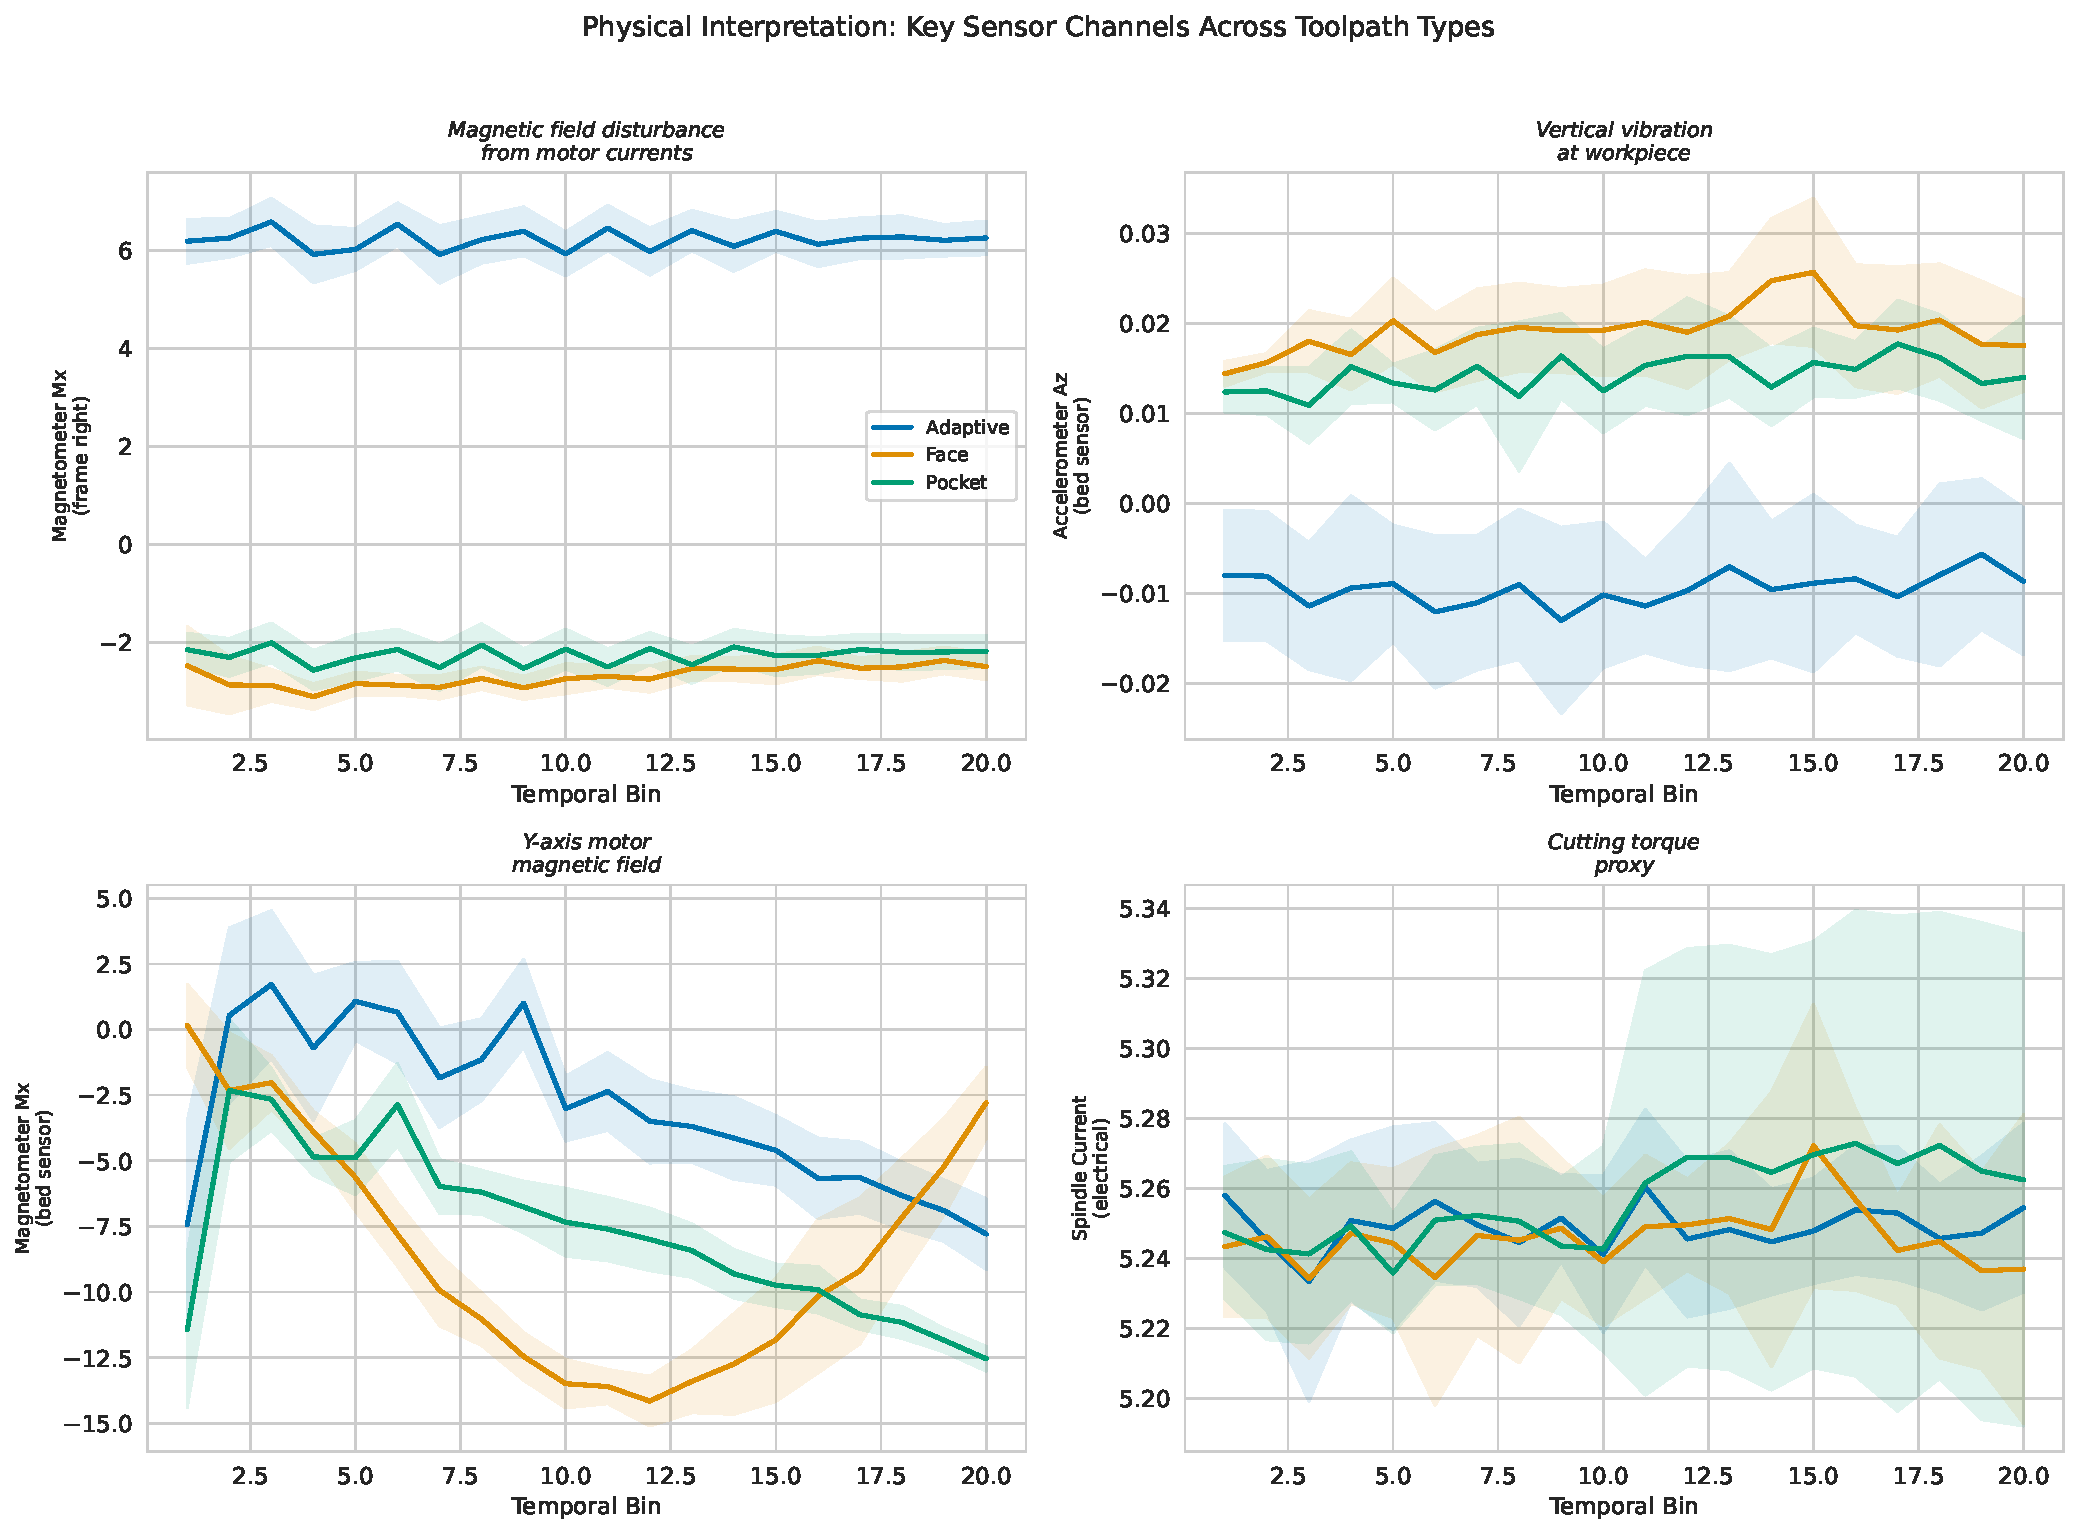
\includegraphics[width=\textwidth]{figures/fig13_physical_interpretation.pdf}
    \caption{Temporal profiles of four physically distinct sensor channels across toolpath types. Top-left: magnetometer Mx on the frame captures a static offset reflecting different workspace regions. Top-right: vertical accelerometer on the bed shows quasi-static motion differences between types (note: at \SI{4}{\hertz} sampling, this captures trajectory dynamics, not cutting vibration). Bottom-left: magnetometer Mx on the bed shows temporal evolution as the table traverses different regions of the machine's static magnetic field. Bottom-right: spindle current is nearly identical across types.}
    \label{fig:physical_interpretation}
\end{figure}

The physical interpretation supports four findings:

\textbf{Magnetometer dominance reflects workspace position, not cutting forces.} The top-ranked feature (frame\_r2.Mx) shows a large static offset between toolpath types: adaptive clearing operates at Mx~$\approx +6.2$ while facing and pocketing sit at Mx~$\approx -2.5$. The three G-code programs traverse different regions of the machine workspace, and we attribute the offset to the local magnetic field differing between those regions, consistent with varying proximity to stepper motor permanent magnets and ferromagnetic structural components. At the \SI{4}{\hertz} effective sampling rate, the magnetometer measures the quasi-static magnetic field at the sensor's position (in effect acting as an indirect position encoder) rather than detecting time-varying fields from motor current waveforms (which would require sampling at $\geq 10\times$ the stepper electrical frequency). While highly discriminative, this signal reflects \emph{program geometry} rather than \emph{cutting dynamics}; it is the sensor-domain analog of the trivial position baseline (Table~\ref{tab:trivial_baselines}).

\textbf{Bed-mounted magnetometer tracks table position.} The y\_bed\_\_3 magnetometer Mx shows strong temporal evolution (temporal CV = 0.4--1.0), with progressive drift that tracks the Y-axis table position as it moves through the machine's static magnetic field landscape. The bed-mounted sensor physically translates with the worktable, and we attribute the drift to its changing proximity to the Y-axis stepper motor's permanent magnets over the toolpath. Under this interpretation, y\_bed\_\_3.Mx is an indirect position encoder for the Y-axis rather than a motor current sensor (which would require bandwidth far above \SI{4}{\hertz}). Different toolpath geometries produce different Y-axis motion profiles, creating distinct temporal magnetic signatures.

\textbf{Spindle current distinguishes cutting from non-cutting but not between toolpath types.} Spindle current is nearly identical across all three active-cutting types (5.245--5.257~A, temporal CV~$< 0.002$). While spindle current rises when the tool engages material (distinguishing active from air cutting), the 0.025'' depth of cut on this desktop CNC produces cutting loads too small relative to the spindle's no-load draw ($\sim$5.2~A at 12{,}000~RPM) to differentiate between toolpath engagement patterns at 4~Hz sampling. Higher cutting depths or higher sampling rates would likely increase this channel's discriminative power.

\textbf{Accelerometer channels capture quasi-static motion differences.} The accelerometer Az on the bed sensor shows distinct temporal profiles per toolpath type, with adaptive clearing most stable and facing showing periodic variations corresponding to pass reversals. However, absolute acceleration differences are small ($\sim$\SI{20}{\milli\g}), which is near the LSM9DS1's bias uncertainty floor (\SI{10}{}--\SI{50}{\milli\g}; see Section~\ref{sec:experimental_setup}). At \SI{4}{\hertz} sampling, these channels measure low-frequency trajectory dynamics and gravitational tilt changes rather than cutting-induced vibration (which occurs at \SI{400}{\hertz}+). Two senses of ``process-relevant'' must be distinguished here. At \SI{4}{\hertz}, the accelerometer features are \emph{trajectory-relevant} (they encode how the machine moves through space during each toolpath) but they are \emph{not force-relevant}, as they do not capture cutting-force-induced vibration. On a higher-bandwidth measurement system, the same accelerometer channels would also capture force signatures, providing a more directly process-physical signal. Their lower importance ranking in this study reflects the small absolute trajectory-dynamics differences compared to the magnetometer's large position-dependent offsets.

Figure~\ref{fig:gcode_phases} annotates the temporal fingerprints with G-code phase information, linking the sensor signal evolution to program structure.

\begin{figure}[H]
    \centering
    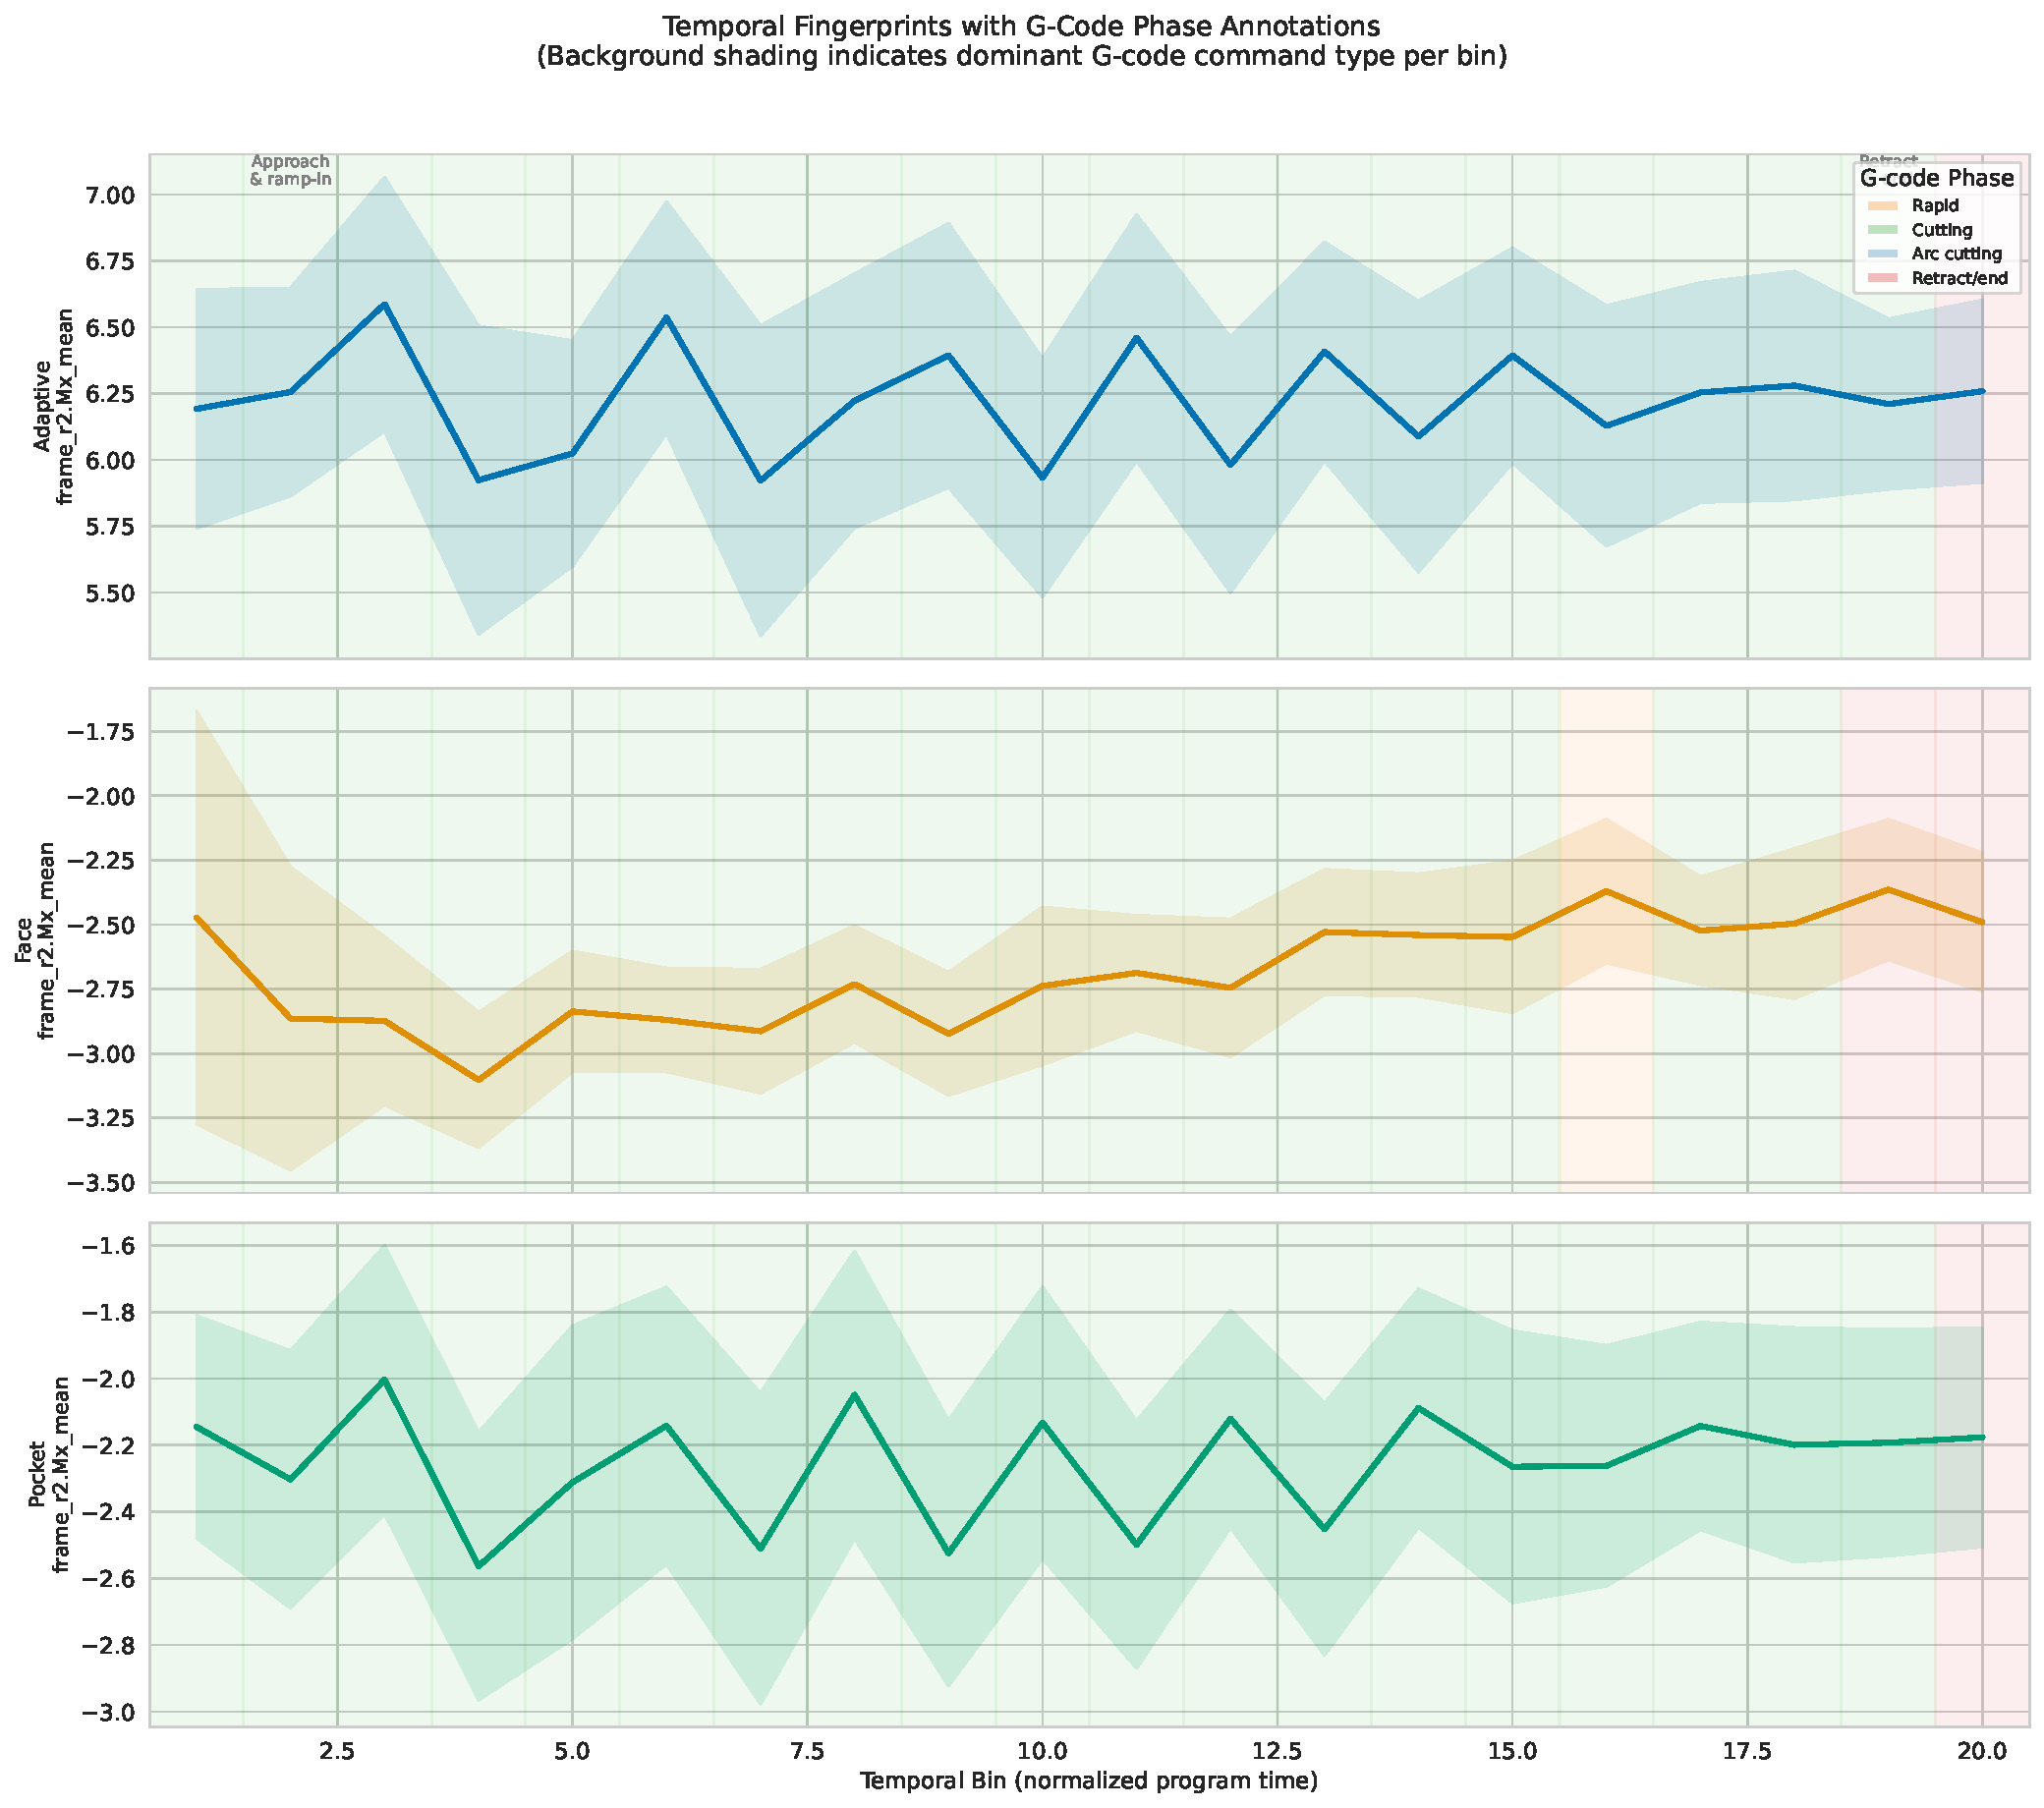
\includegraphics[width=\textwidth]{figures/fig15_gcode_phases.pdf}
    \caption{Temporal fingerprints annotated with G-code phases. Background shading: green = cutting (G1/MOVE), blue = arcs (G2/G3), orange = rapid (G0), red = retract/end (G53/M30). Facing programs terminate early (bins 16--20 are retract/idle), producing a distinctive signal drop.}
    \label{fig:gcode_phases}
\end{figure}

The phase-annotated figure confirms that facing programs terminate earlier (bins 16--20 are retract/idle), producing a distinctive signal drop, while adaptive and pocketing maintain cutting through bin 19. The temporal fingerprint structure directly tracks the G-code program sequence; different programs produce different temporal bin compositions, which drives the classification.

Table~\ref{tab:temporal_cv} quantifies the temporal variability of each key sensor channel across toolpath types. Channels with high temporal coefficient of variation (CV) exhibit strong temporal structure that could encode either process dynamics or program geometry; channels with low CV are temporally flat.

\begin{table}[H]
\caption{Temporal variability of key sensor channels across toolpath types. Temporal CV is the coefficient of variation of the channel's mean across the 20 temporal bins; higher values indicate stronger temporal structure. Range is the bin-to-bin dynamic range.}\label{tab:temporal_cv}
\centering
\small
\begin{tabular}{llccc}
\toprule
\textbf{Channel} & \textbf{Toolpath} & \textbf{Mean} & \textbf{Temporal CV} & \textbf{Range} \\
\midrule
\multirow{3}{*}{frame\_r2.Mx (position proxy)} & Adaptive & $+6.22$ & 0.032 & 0.67 \\
& Facing & $-2.68$ & 0.076 & 0.74 \\
& Pocket & $-2.25$ & 0.074 & 0.56 \\
\midrule
\multirow{3}{*}{y\_bed\_\_3.Mx (Y-axis position)} & Adaptive & $-2.99$ & 1.000 & 9.50 \\
& Facing & $-8.43$ & 0.526 & 14.30 \\
& Pocket & $-7.73$ & 0.397 & 10.21 \\
\midrule
\multirow{3}{*}{y\_bed\_\_3.Az (cutting vibration)} & Adaptive & $-0.009$ & 0.184 & 0.007 \\
& Facing & $+0.019$ & 0.135 & 0.011 \\
& Pocket & $+0.014$ & 0.128 & 0.007 \\
\midrule
\multirow{3}{*}{spindle2.RMS (vibration energy)} & Adaptive & 5{,}762 & 0.311 & 7{,}227 \\
& Facing & 7{,}167 & 0.316 & 8{,}475 \\
& Pocket & 5{,}351 & 0.328 & 6{,}611 \\
\midrule
\multirow{3}{*}{spindle current (cutting torque)} & Adaptive & 5.249 & 0.001 & 0.027 \\
& Facing & 5.246 & 0.002 & 0.038 \\
& Pocket & 5.257 & 0.002 & 0.037 \\
\bottomrule
\end{tabular}
\end{table}

The table reveals two physically distinct discrimination mechanisms: (1)~the frame\_r2.Mx magnetometer separates toolpath types via \emph{static offset} (mean values differ by $\sim$9 units between adaptive and face/pocket) with minimal temporal structure (CV~$< 0.08$); and (2)~the y\_bed\_\_3.Mx magnetometer and spindle2.RMS channels separate types via \emph{temporal dynamics} (CV~$> 0.3$) with different temporal evolution patterns. The spindle current, despite being the most direct proxy for cutting torque, provides neither offset-based nor dynamics-based discrimination (CV~$< 0.002$, range~$< 0.04$~A).

\subsubsection{Effect of Air-Cut Referencing on Feature Confounds}

We next test whether air-cut subtraction removes the workspace-position confound. Table~\ref{tab:confound_removal} compares the channel-type distribution of top features between the raw and subtracted isolation methods.

\begin{table}[H]
\caption{Distribution of channel types among the top 20 most important features, for raw vs.\ subtracted isolation. Air-cut subtraction reduces magnetometer dominance from 61\% to 21\% of feature importance, shifting weight toward electrical and environmental channels.}\label{tab:confound_removal}
\centering
\begin{tabular}{lcc}
\toprule
\textbf{Channel Type} & \textbf{Raw (top 20)} & \textbf{Subtracted (top 20)} \\
\midrule
Magnetometer     & 12 features (61.0\%) & 4 features (20.8\%) \\
Environmental    & 3 features           & 6 features \\
Color            & 2 features           & 2 features \\
Electrical       & 0 features           & 4 features \\
Accelerometer    & 1 feature            & 1 feature \\
Other            & 2 features           & 3 features \\
\bottomrule
\end{tabular}
\end{table}

Air-cut subtraction reduces the magnetometer's share of the top 20 features from 61\% (raw) to 21\% (subtracted), and elevates electrical motor current features from 0 to 4 of the top 20. We attribute this shift to the air-cut reference capturing a similar workspace trajectory, so that subtracting it partially removes position-dependent magnetic field offsets. The remaining discriminative signal is more likely to reflect motor load and quasi-static motion differences rather than workspace geometry.

\subsubsection{Classification Without Position-Confounded Channels}

To directly assess how much classification accuracy depends on position-confounded channels (magnetometer, color, proximity, pressure) versus channels that respond to machine dynamics (accelerometer, gyroscope, RMS, electrical), Table~\ref{tab:confound_controlled} reports accuracy when confounded channels are progressively excluded.

\begin{table}[H]
\caption{Classification accuracy (RF, 20$\times$5 repeated CV) when position-confounded channels are progressively excluded. Removing all magnetometers drops accuracy only to 96.1\%; accelerometer-only features still reach 93.0\%, while the true electrical-only set (the 8 current channels, 112 features) is the weakest group at 76.5\%. Backing artifact: \texttt{experiment\_confound\_controlled.json}.}\label{tab:confound_controlled}
\centering
\begin{tabular}{lcc}
\toprule
\textbf{Channel Configuration} & \textbf{Accuracy (\%)} & \textbf{Features} \\
\midrule
All channels                                  & $98.9 \pm 3.1$ & 1{,}540 \\
No magnetometers (Mx, My, Mz removed)       & $96.1 \pm 5.4$  & 1{,}288 \\
No mag + color + pressure + proximity        & $96.7 \pm 4.8$  & 784 \\
Accel + gyro + RMS + temperature only        & $95.1 \pm 6.1$  & 672 \\
Accelerometer + gyroscope only               & $94.4 \pm 6.3$  & 504 \\
Accelerometer only                           & $93.0 \pm 6.3$  & 252 \\
Electrical current only (no IMU)             & $76.5 \pm 12.4$ & 112 \\
\bottomrule
\end{tabular}
\end{table}

Three findings emerge: (1)~removing all magnetometers drops accuracy by only $\sim$3 percentage points (98.9\% $\to$ 96.1\%), confirming that while magnetometers dominate feature importance, they are not essential; (2)~accelerometer and gyroscope channels alone achieve 94.4\%, demonstrating that quasi-static motion dynamics carry sufficient discriminative information independent of position confounds; and (3)~the electrical-current channels alone are the weakest group (76.5\%), consistent with their low between-class SNR (the per-channel SNR budget below), whereas the motion-dynamics channels (accel/gyro/RMS/temperature, 95.1\%) retain almost all of the discriminative signal. (An earlier version of this table reported the electrical group at 96.0\%/350 features; that figure was inflated by the same \texttt{spindle}$\to$\texttt{spindle2} feature leak corrected above, which had folded IMU channels into the ``electrical'' set.)

\subsubsection{Full Pipeline Without Magnetometers}

To test whether air-cut referencing provides value beyond position encoding, we re-run the complete pipeline using only non-confounded channels (accelerometer, gyroscope, RMS, temperature, and the eight electrical-current channels; 784 features, excluding all magnetometer, color, pressure, and proximity channels; Table~\ref{tab:nomag_pipeline}).

\begin{table}[H]
\caption{Repeated CV (20$\times$5-fold) with confound-free features only (784 features, no magnetometers/color/pressure/proximity). The subtracted and ratio methods hold 100\% across all 100 folds; z-score remains near-perfect (99.0\%, min 90\%); raw degrades to 96.7\%.}\label{tab:nomag_pipeline}
\centering
\begin{tabular}{llcccc}
\toprule
\textbf{Method} & \textbf{Clf} & \textbf{Mean (\%)} & \textbf{Std} & \textbf{Min (\%)} & \textbf{Max} \\
\midrule
Raw        & RF  & 96.7 & 4.8 & 81.8 & 100.0 \\
Subtracted & RF  & 100.0 & 0.0 & 100.0 & 100.0 \\
Ratio      & RF  & 100.0 & 0.0 & 100.0 & 100.0 \\
Z-score    & RF  & 99.0 & 2.9 & 90.0 & 100.0 \\
\midrule
Raw        & MLP & 79.9 & 17.0 & 20.0 & 100.0 \\
Z-score    & MLP & 90.0 & 13.0 & 36.4 & 100.0 \\
\bottomrule
\end{tabular}
\end{table}

With all position-confounded channels removed, raw RF features degrade to 96.7\% mean accuracy (minimum fold 81.8\%), while \textbf{the subtracted and ratio methods maintain perfect 100\% accuracy across all 100 evaluations and z-score remains near-perfect at 99.0\% (minimum fold 90\%)}. The effect is larger for the noise-sensitive MLP, where raw reaches only 79.9\% and z-score recovers to 90.0\%. This demonstrates that air-cut referencing provides a genuine classification benefit that is independent of the magnetometer position-encoding confound identified in Section~\ref{sec:physics}. On this confound-free set, however, the benefit is a few percentage points and a variance reduction (subtracted/ratio reaching the ceiling) rather than the uniform jump to 100\% observed when position-confounded channels are present.\footnote{Temperature is retained in this ``confound-free'' set despite showing run-order correlation $r = 0.98$ within the adaptive class (Section~\ref{sec:discussion}). Temperature is a within-class drift effect, not a between-class confound, so it remains a defensible process-relevant channel. A stricter definition excluding temperature does not materially change the results.}

Noise robustness was also re-evaluated on the 784-feature confound-free set: subtracted features maintain 100\% accuracy up to $0.5\times$ additive noise and 99.0\% at $1.0\times$ noise, while raw features drop to 91.2\% at $1.0\times$ and 71.3\% at $2.0\times$. The robustness advantage persists when position-confounded channels are excluded, confirming that air-cut referencing improves resilience to feature-level perturbations on the underlying motion-dynamics signal.

\subsection{Damaged-Spindle Detection: A Position-Controlled Task}\label{sec:damage}

The experiments above isolate the process-relevant signal by \emph{removing} position-confounded channels. A complementary and stronger test instead holds workspace position \emph{constant} while varying only the process. We use the vetted set of damaged-spindle runs: 14 air-cut runs (5/4/5 for adaptive/facing/pocketing) that execute the same CAM toolpath strategies with one spindle drive band removed to induce spindle runout. The toolpath geometry, and hence the workspace region, matches the normal runs, so workspace position provides little separation between the normal-vs-damaged labels. Because the damaged runs are air-cuts and the normal runs are active cuts, however, the process difference couples two factors: spindle condition (runout) and cutting engagement (material load). This is the within-region test that the magnetometer position-encoder cannot solve; it demonstrates process-dynamics detection under position control, but the coupled design means it does not by itself validate tool-condition monitoring.

We pool the 51 normal active runs (the same vetted set used throughout the paper) and the 14 damaged-spindle runs into a binary task (majority-class baseline 78.5\%) and classify with the same RF temporal-binning pipeline under 20$\times$5-fold repeated CV (Table~\ref{tab:damage}).

\begin{table}[H]
\caption{Damaged-spindle detection (binary: 51 normal active vs.\ 14 damaged-spindle air-cut runs, same toolpath strategies). Mean over 20$\times$5-fold repeated CV; majority-class baseline 78.5\%. Per-type accuracy (same program, workspace held constant): adaptive 100\%, facing 100\%, pocketing 100\%.}\label{tab:damage}
\centering
\begin{tabular}{lccc}
\toprule
\textbf{Method} & \textbf{Accuracy (\%)} & \textbf{$F_1$ (damage)} & \textbf{Balanced Acc.} \\
\midrule
Raw        & $98.5 \pm 3.1$ & 0.970 & 0.990 \\
Subtracted & $98.5 \pm 3.1$ & 0.970 & 0.990 \\
\bottomrule
\end{tabular}
\end{table}

Random Forest reaches 98.5\% accuracy (balanced accuracy 0.990, damage-class $F_1 = 0.97$), far above the 78.5\% majority baseline, and per-type accuracy is 100\% for all three toolpath types, where the same program holds the workspace constant. Two findings follow. First, the discriminative signal shifts almost entirely away from position. The channel-type importance (from a Random Forest fit on the full set) is now dominated by the \textbf{accelerometer (44.7\%)} and \textbf{acoustic RMS (29.6\%)}, process-dynamics channels amounting to $\sim$74\% combined, with the magnetometer contributing only \textbf{0.1\%}, versus the 61\% of top-20 feature importance it commanded on the position-confounded three-class task (Section~\ref{sec:physics}). Spindle runout and the absence of cutting engagement both perturb the vibration and acoustic signature; this design cannot attribute the separation to either factor alone. Second, air-cut referencing is \emph{neutral} here (raw and subtracted both 98.5\%). When workspace position is already held constant there is no position-dependent offset for the air-cut baseline to remove, as the causal model (Section~\ref{sec:causal_dag}) predicts; referencing helps when the position confound is present and is neither beneficial nor harmful when it is absent. The dataset is small (14 damaged-spindle runs from a single session), so this is a demonstration rather than a validated detector; but it establishes that the sensor array does carry process-relevant information, recoverable once the position confound is controlled. The clean damage-only comparison, damaged-spindle air-cuts against normal air-cuts of the same programs, is left to future work.

\subsection{Permutation Test}

A permutation test with 1{,}000 label shuffles using the full 1{,}540-feature set (raw isolation method, RF classifier) confirms that the classification result is non-random. The null distribution has mean accuracy $35.2\% \pm 8.2\%$ (close to the random baseline of $33.3\%$) with a maximum of 62.7\%, far below the observed 100\% ($p < 0.001$). This rules out the possibility that the classification result is an artifact of overfitting on the small sample size.

\subsection{Effective Dimensionality}

Despite the nominal 1{,}540-feature space (30:1 feature-to-sample ratio), PCA analysis reveals that 7 components explain 50\% of variance and 30 components explain 90\%. The effective dimensionality is high relative to the sample count ($n = 51$), but only 0.15\% of feature pairs have $|r| > 0.95$, indicating moderate rather than extreme redundancy. The RF classifier's success at full dimensionality, combined with its degradation under PCA (Section~\ref{sec:ablation}), suggests it exploits many individually weak but collectively informative features, a regime where tree-based ensembles excel.

\subsection{Internal Held-Out Split (Same Session)}

To complement the cross-validation analysis, we performed a single internal held-out split: 12 of the 51 active-cutting runs (4 per class) were withheld from all training and CV operations and evaluated only once at the end, with the air-cut baseline statistics ($\boldsymbol{\mu}_\text{air}$, $\boldsymbol{\sigma}_\text{air}$) and the PCA transform fit only on the 39 training runs. These 12 runs are drawn from the same 51-run, same-machine, same-session dataset, so this is a guard against fold-reuse leakage rather than an independent generalization test. Table~\ref{tab:heldout} reports the held-out accuracy for each isolation method.

\begin{table}[H]
\caption{Internal held-out split accuracy. 12 runs (4 per class) randomly stratified from the same 51 active-cutting runs (same machine/session), evaluated once after training (including the air-cut baseline and PCA) on the remaining 39.}\label{tab:heldout}
\centering
\begin{tabular}{lccc}
\toprule
\textbf{Method} & \textbf{Test Accuracy} & \textbf{$n_{\text{train}}$} & \textbf{$n_{\text{test}}$} \\
\midrule
Raw        & 100.0\% & 39 & 12 \\
Subtracted & 100.0\% & 39 & 12 \\
Ratio      & 100.0\% & 39 & 12 \\
Z-score    & 100.0\% & 39 & 12 \\
\bottomrule
\end{tabular}
\end{table}

All four methods achieve 100\% accuracy on this internal split, indicating the cross-validation results are not artifacts of fold-reuse or data reuse across splits. Because the 12 runs share the same machine, session, and CAM programs as the training runs, this is \emph{not} evidence of cross-session or cross-machine generalization (see Section~\ref{sec:discussion} Limitations); with $n = 12$ and a single split it is also a coarse estimate.

\subsection{Per-Channel SNR Budget}

To quantify which sensor types carry the most discriminative information independent of feature-importance rankings, we compute a between-class versus within-class variance ratio (signal-to-noise ratio, SNR) for each of the 1{,}540 features. Table~\ref{tab:snr_budget} reports median and maximum SNR by channel type.

\begin{table}[H]
\caption{Per-channel SNR budget. SNR is computed as $10\log_{10}(\sigma^2_{\text{between-class}} / \sigma^2_{\text{within-class}})$ in dB. Magnetometer channels have the highest median and max SNR, consistent with the position-confound finding.}\label{tab:snr_budget}
\centering
\begin{tabular}{lcccc}
\toprule
\textbf{Channel Type} & \textbf{Median SNR (dB)} & \textbf{Max SNR (dB)} & \textbf{N features} \\
\midrule
Magnetometer    & $-3.7$  & $24.2$ & 252 \\
Vibration RMS   & $-4.2$  & $2.8$  & 84 \\
Accelerometer   & $-7.6$  & $11.7$ & 252 \\
Temperature     & $-7.9$  & $1.9$  & 84 \\
Proximity       & $-8.1$  & $4.5$  & 84 \\
Gyroscope       & $-8.3$  & $6.1$  & 252 \\
Pressure        & $-8.8$  & $11.7$ & 84 \\
Color           & $-9.0$  & $14.3$ & 336 \\
Electrical      & $-11.0$ & $3.7$  & 112 \\
\bottomrule
\end{tabular}
\end{table}

Magnetometer channels achieve the highest median SNR ($-3.7$~dB) and max SNR ($24.2$~dB), with the top 6 highest-SNR features all being magnetometer (Mx, Mz) channels from the frame\_r2 sensor. This quantitatively confirms the position-encoding finding from Section~\ref{sec:physics}: the channels with the largest signal-to-noise ratio for class discrimination are those most affected by workspace position. Accelerometer and gyroscope channels have negative median SNR (within-class variance exceeds between-class variance for typical features), reflecting the within-class variability of the trajectory dynamics they capture. Electrical current channels have the lowest median SNR ($-11.0$~dB), consistent with their near-constant behavior under shallow UHMW-PE cutting.

\subsection{Run-Order Confound Analysis}

Section~\ref{sec:discussion} reports that several features show statistically significant temporal drift correlated with run order (e.g., temperature, $r = 0.98$ for adaptive class). To verify that this within-class drift does not confound the between-class classification, we compute the partial correlation between each top-importance feature and the class label, controlling for run order. Across the top 20 features, the partial correlations differ from the raw correlations by an average of $-1.7\%$ (with several features showing slightly stronger partial correlations, indicating that run order is not aliased with class). This rules out run-order temporal drift as an explanation for the classification results. The class signal in these features is essentially independent of when each run was collected.

\subsection{Fine-Grained Learning Curve}

Figure~\ref{fig:learning_curve_fine} extends the learning curve analysis (Section~\ref{sec:ablation}) with finer resolution at small training-set sizes, where the air-cut referencing benefit is most pronounced.

\begin{figure}[H]
    \centering
    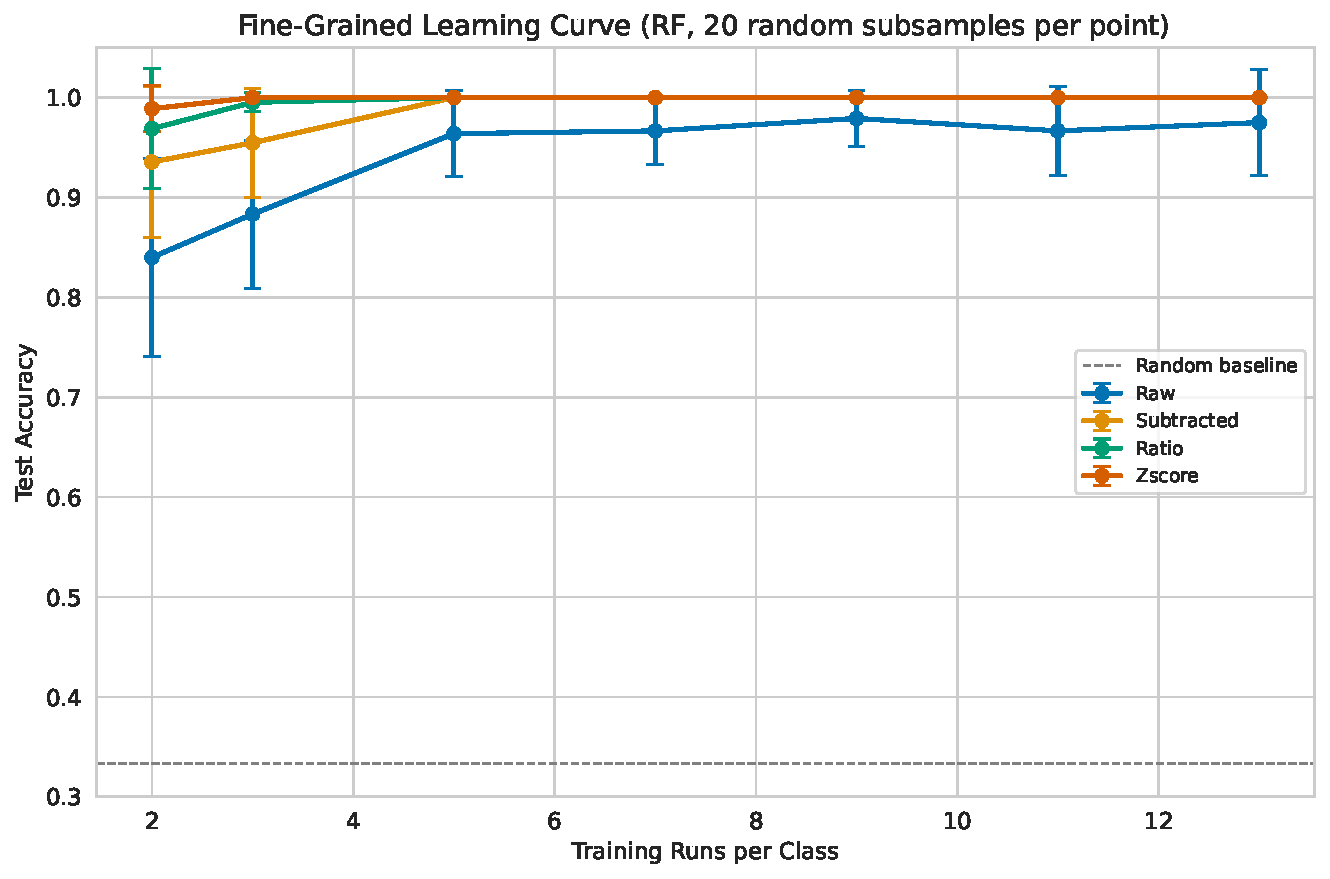
\includegraphics[width=0.85\textwidth]{figures/fig19_learning_curve_fine.pdf}
    \caption{Fine-grained learning curve: classification accuracy vs.\ training runs per class for all four isolation methods (RF, 10 random subsamples per point). Z-score referencing achieves 98.9\% with only 2 training runs per class, while raw features need many more runs to match.}
    \label{fig:learning_curve_fine}
\end{figure}

With only \textbf{2 runs per class} (6 training samples total), z-score referencing achieves 98.9\% accuracy, ratio achieves 96.9\%, subtracted achieves 93.6\%, and raw features lag at 84.0\%. Air-cut referencing therefore improves data efficiency; the accuracy that raw features require ${\sim}10$ training runs to reach, z-score achieves with only 2. For applications where labeled training data is expensive (e.g., destructive testing or high-volume production), this difference is practically meaningful.

\subsection{Calibration Analysis}

Beyond classification accuracy, model calibration (whether predicted probabilities match observed accuracy) matters for downstream decision-making. Table~\ref{tab:calibration} reports Expected Calibration Error (ECE) and log loss across the four isolation methods.

\begin{table}[H]
\caption{Calibration metrics. ECE = Expected Calibration Error (10 bins). Lower is better-calibrated. All methods achieve 100\% accuracy; calibration differences reflect prediction confidence patterns.}\label{tab:calibration}
\centering
\begin{tabular}{lccc}
\toprule
\textbf{Method} & \textbf{ECE} & \textbf{Log Loss} & \textbf{Mean Confidence} \\
\midrule
Raw        & 0.119 & 0.135 & 0.881 \\
Subtracted & 0.078 & 0.083 & 0.923 \\
Ratio      & 0.084 & 0.090 & 0.916 \\
Z-score    & \textbf{0.077} & \textbf{0.083} & 0.923 \\
\bottomrule
\end{tabular}
\end{table}

Air-cut referenced methods achieve $\sim$35\% lower ECE than raw features (0.077--0.084 vs.\ 0.119) and lower log loss, indicating better-calibrated probability estimates. The mean prediction confidence is also higher for referenced methods ($\sim$0.92 vs.\ 0.88), meaning the classifier is more decisive when air-cut referencing is applied. Well-calibrated probabilities enable confidence-thresholding for novelty detection and selective abstention, which gives this calibration improvement practical value.

\subsection{MiniRocket Comparison}

To benchmark against a state-of-the-art time-series classification method, we apply MiniRocket~\cite{dempster2020rocket} (the deterministic variant of ROCKET using fixed length-9 kernels with weights from $\{-1, 2\}$) to the raw downsampled sensor time series.

\begin{table}[H]
\caption{Comparison against MiniRocket-style features (12 fixed kernels $\times$ 110 channels = 1{,}320 features) on downsampled raw time series.}\label{tab:minirocket}
\centering
\begin{tabular}{lcc}
\toprule
\textbf{Method} & \textbf{Accuracy} & \textbf{Features} \\
\midrule
MiniRocket + RF      & $96.2\% \pm 4.7$ & 1{,}320 \\
MiniRocket + Ridge   & $96.0\% \pm 8.0$ & 1{,}320 \\
\midrule
Temporal binning + RF (ours, full)  & $100.0\% \pm 0.0$ & 1{,}540 \\
Temporal binning + RF (confound-free, referenced) & $100.0\% \pm 0.0$ & 784 \\
\bottomrule
\end{tabular}
\end{table}

MiniRocket achieves 96\% accuracy, comparable to but slightly below our temporal binning approach. This benchmark places our method within the competitive range of modern time-series classification techniques while preserving interpretability through explicit per-bin statistics, sensor-channel attribution, and physical analysis of dominant features, advantages that random convolutional kernel methods do not provide.

\subsection{Visual Comparison: Full vs.\ Confound-Free Pipeline}

Figure~\ref{fig:confound_free_viz} visualizes the full classification accuracy comparison across all four isolation methods, three classifiers, and two feature sets (full 1{,}540 features vs.\ 784 confound-free features).

\begin{figure}[H]
    \centering
    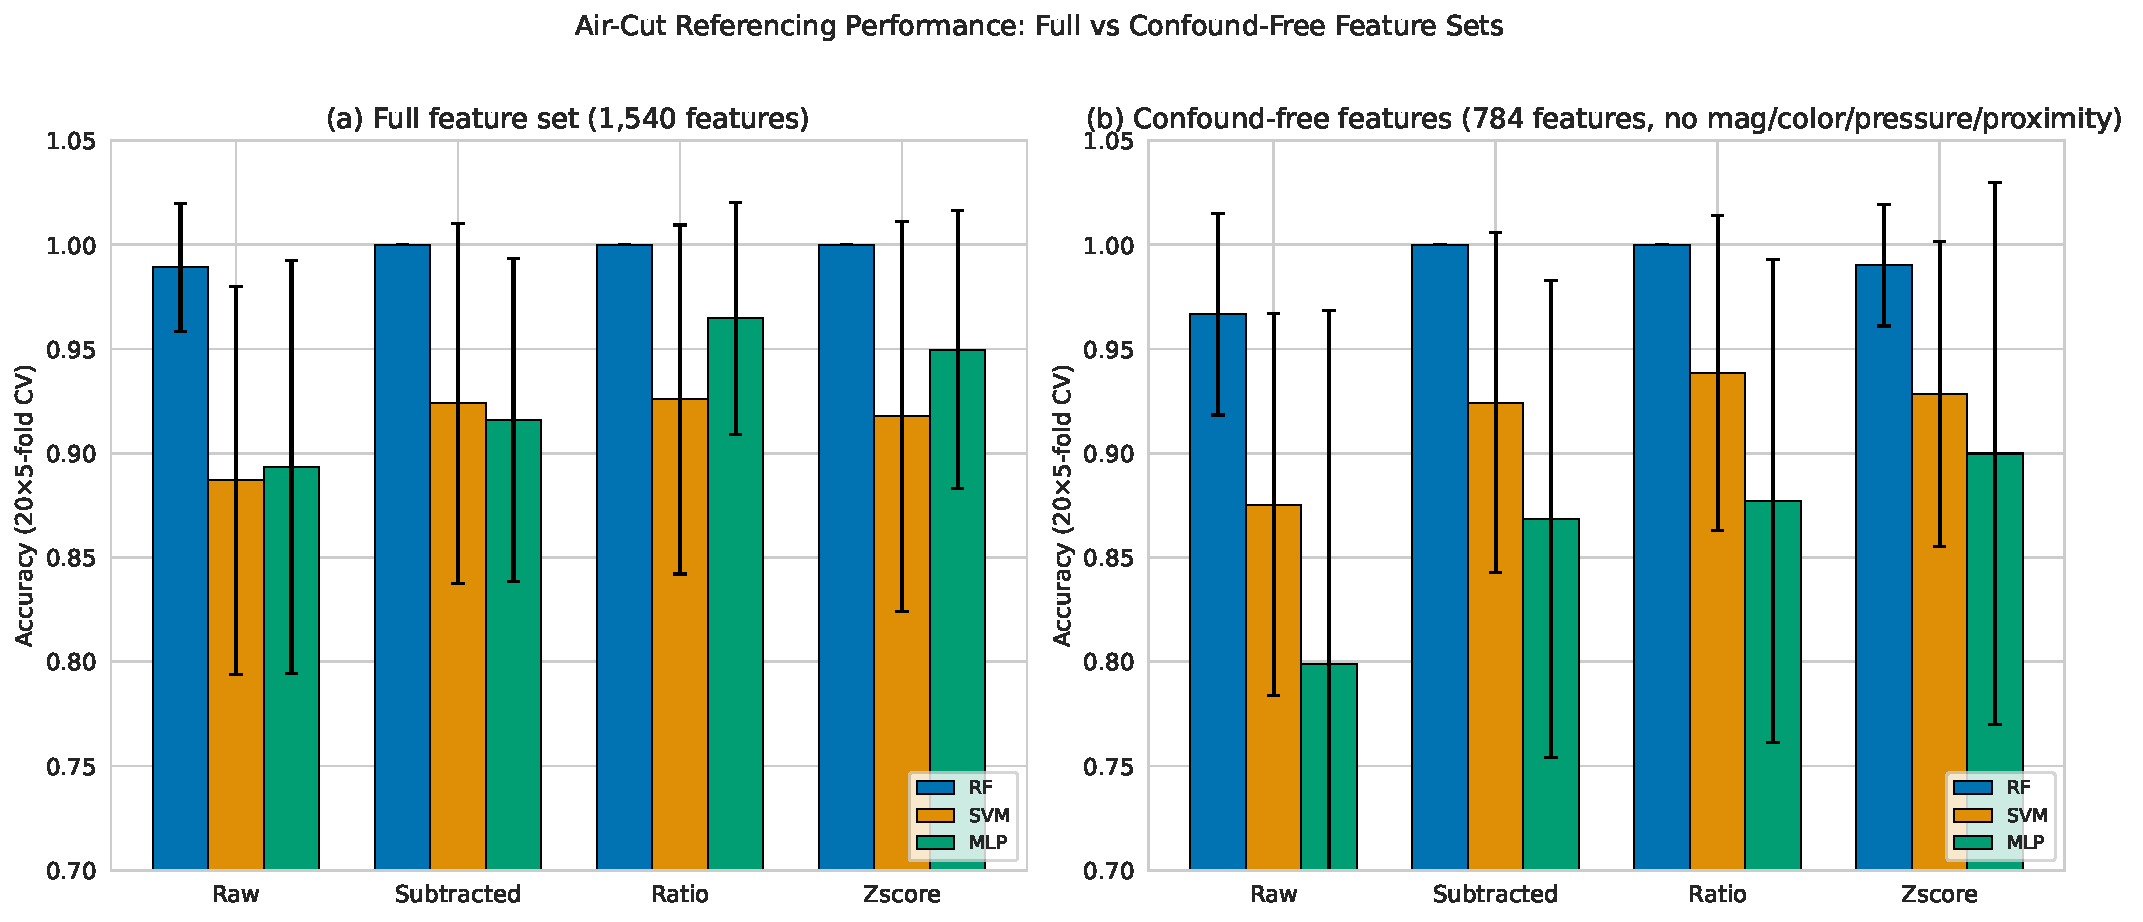
\includegraphics[width=\textwidth]{figures/fig20_confound_free_comparison.pdf}
    \caption{Air-cut referencing performance comparison. Left: full 1{,}540-feature set including position-confounded magnetometer channels. Right: 784 confound-free features (no magnetometer, color, pressure, proximity). The raw-vs-referenced gap widens in the confound-free condition, particularly for SVM and MLP, demonstrating that referencing provides genuine benefit beyond position encoding. (Panel regenerated on the corrected 784-feature set; subtracted/ratio RF reach 100\% and z-score RF 99.0\%, vs.\ raw 96.7\%.)}
    \label{fig:confound_free_viz}
\end{figure}

In the confound-free condition (right panel), the gap between raw and referenced methods widens. For RF, raw drops from $\sim$99\% to 96.7\% while the subtracted and ratio methods stay at 100\% and z-score at 99.0\%. For MLP, raw drops to $\sim$80\% while z-score recovers to 90\%. The position-confounded channels were inflating the raw baseline; removing them reveals the true (more modest) magnitude of the air-cut referencing benefit.

\subsection{Mutual Information Decomposition}\label{sec:mi}

To quantify how much of each feature's discriminative content is genuinely class-related versus position-encoded, we compute mutual information (MI) between each feature and three targets: the class label, the run order, and a position proxy defined as the first principal component of the magnetometer feature subspace. The position proxy explains 21.2\% of magnetometer variance and serves as a continuous proxy for the workspace region traversed during a run.

\begin{table}[H]
\caption{Mutual information by sensor channel type. MI is reported in bits; the maximum possible MI between a feature and a 3-class label is $\log_2 3 = 1.585$ bits. The ``\%pos/cls'' column reports the ratio of position-MI to class-MI, where values near or above 100\% indicate that the feature's class-discriminative content is fully accounted for by workspace position.}\label{tab:mi_decomposition}
\centering
\begin{tabular}{lccccc}
\toprule
\textbf{Channel Type} & \textbf{MI(class)} & \textbf{MI(order)} & \textbf{MI(pos)} & \textbf{\%pos/cls} & \textbf{N} \\
\midrule
Magnetometer  & 0.455 & 0.110 & 0.503 & 110.5\% & 252 \\
Accelerometer & 0.247 & 0.109 & 0.305 & 123.3\% & 252 \\
Gyroscope     & 0.225 & 0.129 & 0.257 & 114.2\% & 252 \\
Vibration RMS & 0.517 & 0.078 & 0.574 & 111.1\% & 84 \\
Temperature   & 0.241 & 0.325 & 0.256 & 106.2\% & 84 \\
Pressure      & 0.538 & 0.153 & 0.431 & 80.0\%  & 84 \\
Proximity     & 0.326 & 0.273 & 0.337 & 103.2\% & 84 \\
Color         & 0.323 & 0.204 & 0.340 & 105.4\% & 336 \\
Electrical    & 0.179 & 0.024 & 0.180 & 100.3\% & 112 \\
\bottomrule
\end{tabular}
\end{table}

\begin{figure}[H]
    \centering
    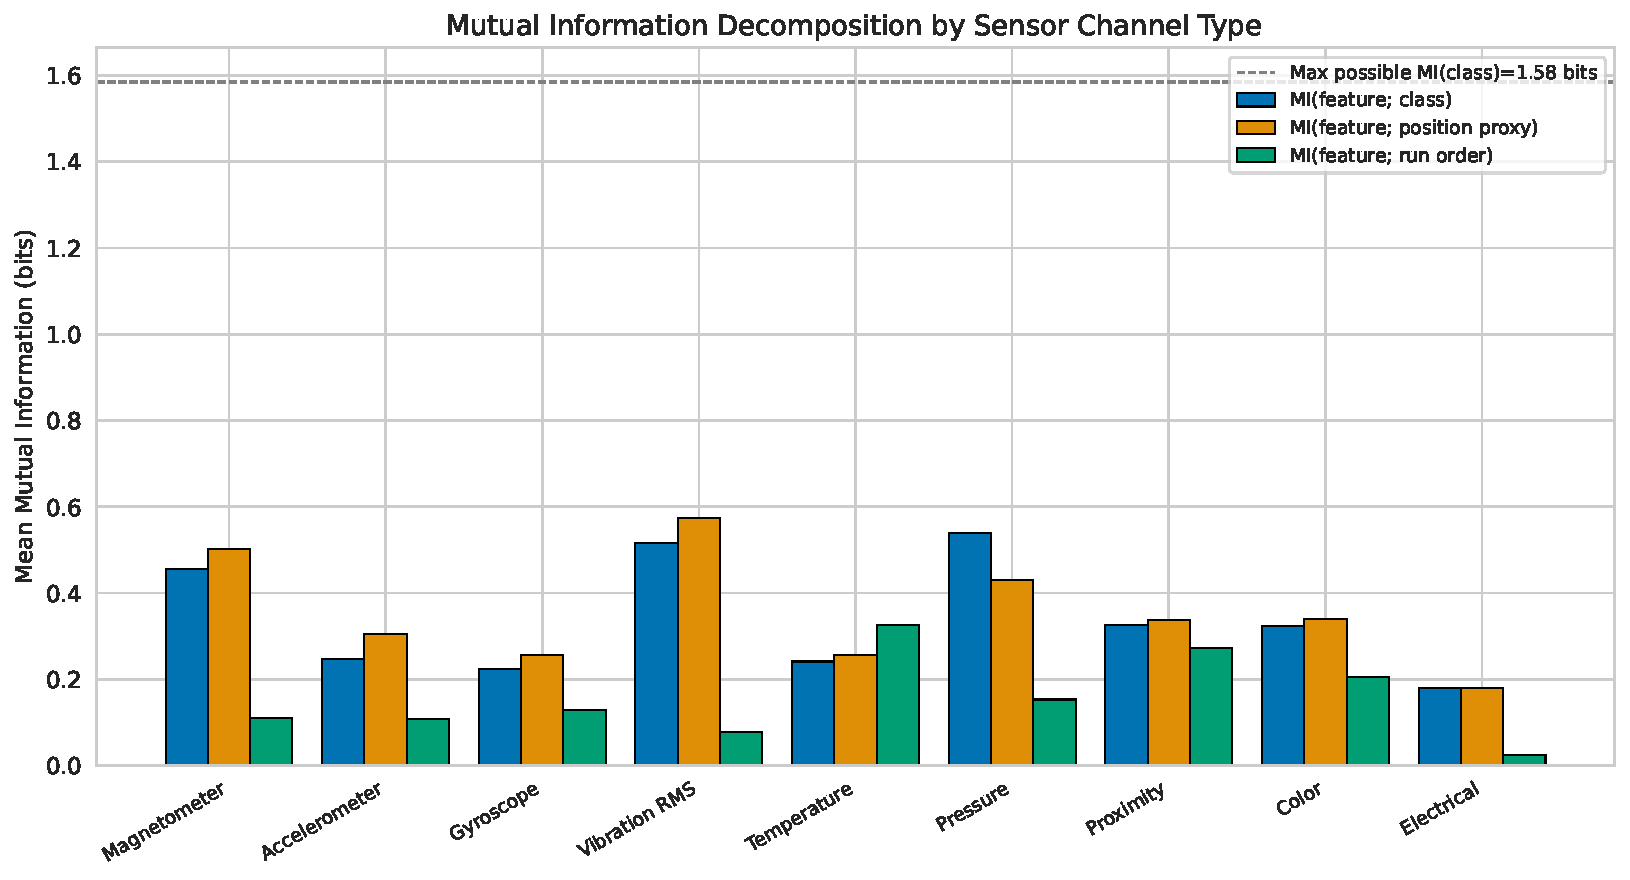
\includegraphics[width=0.85\textwidth]{figures/fig22_mi_decomposition.pdf}
    \caption{Mutual information decomposition by sensor channel type. For nearly all sensor types, MI(feature; position proxy) is comparable to or exceeds MI(feature; class), indicating that workspace position accounts for the majority of class-discriminative content.}
    \label{fig:mi_decomposition}
\end{figure}

The MI analysis quantitatively confirms the position-encoding finding from Section~\ref{sec:physics}. For nearly every channel type, MI(feature; position) is comparable to or exceeds MI(feature; class), with ratios above 100\% indicating that position information saturates the class signal. Pressure (the only ratio below 100\%) carries class information beyond position, but this reflects barometric session-day variation rather than process physics. Of the 1{,}540 features, 362 have MI(class) $> 0.5$~bits, 422 have MI(position) $> 0.5$~bits, and \textbf{321 of those (89\%) overlap}, meaning that the vast majority of high-class-information features are also high-position-information features. Temperature has the highest MI(order) value (0.325 bits), reflecting the within-class warming drift identified in Section~\ref{sec:discussion}; this is one of the few channels where information is genuinely tied to recording chronology rather than class structure or position.

One methodological caveat applies. The position proxy is defined as the first principal component of the magnetometer feature subspace, which makes the MI(magnetometer feature; position) measurement slightly circular by construction (the magnetometer features are partly being correlated with a transformation of themselves). This circularity inflates the magnetometer ratio (110.5\%) by an unknown amount. The more consequential cross-sensor finding is unaffected, however: accelerometer (123.3\%), gyroscope (114.2\%), vibration RMS (111.1\%), proximity (103.2\%), color (105.4\%), and electrical (100.3\%) channels all exceed the 100\% threshold despite being computed independently of the magnetometer subspace, demonstrating that workspace position dominates the discriminative content across the entire sensor array.

\subsection{Bayesian Posterior Analysis}\label{sec:bayesian}

The frequentist analyses (Friedman test, bootstrap CIs, Cliff's delta) provide significance testing under various assumptions, but each is constrained by the ceiling effects in the referenced methods (which achieve 100\% on every fold). To complement these, we model the per-fold accuracy as a Beta-Binomial conjugate problem: with 100 cross-validation folds totaling 1{,}020 test predictions per method, we compute the posterior $\text{Beta}(1 + n_\text{correct}, 1 + n_\text{incorrect})$ on the underlying accuracy, then sample 100{,}000 draws to compute posterior probabilities of difference. The $\text{Beta}(1, 1)$ prior is uniform on $[0, 1]$ and is therefore non-informative; with $n = 1{,}020$ predictions per method, the posterior is dominated by the likelihood and the choice of prior has negligible effect (sensitivity to a Jeffreys $\text{Beta}(0.5, 0.5)$ prior shifts the posterior medians by $< 0.05$ percentage points).

\begin{table}[H]
\caption{Bayesian posterior analysis (Beta-Binomial conjugate, $\text{Beta}(1, 1)$ prior). For each method, $n_\text{correct}/n_\text{total}$ across 100 CV folds gives the likelihood. Posterior 95\% credible intervals (CrI) and posterior probability of exceeding raw are computed from 100{,}000 samples.}\label{tab:bayesian}
\centering
\begin{tabular}{lcccc}
\toprule
\textbf{Method} & \textbf{$n_\text{correct}/n_\text{total}$} & \textbf{Posterior median} & \textbf{95\% CrI} & \textbf{$P(>\text{raw})$} \\
\midrule
Raw        & 1009/1020 & 98.86\% & [98.08\%, 99.39\%] & --- \\
Subtracted & 1020/1020 & 99.93\% & [99.64\%, 100.00\%] & 0.9997 \\
Ratio      & 1020/1020 & 99.93\% & [99.63\%, 100.00\%] & 0.9998 \\
Z-score    & 1020/1020 & 99.93\% & [99.64\%, 100.00\%] & 0.9998 \\
\bottomrule
\end{tabular}
\end{table}

\begin{figure}[H]
    \centering
    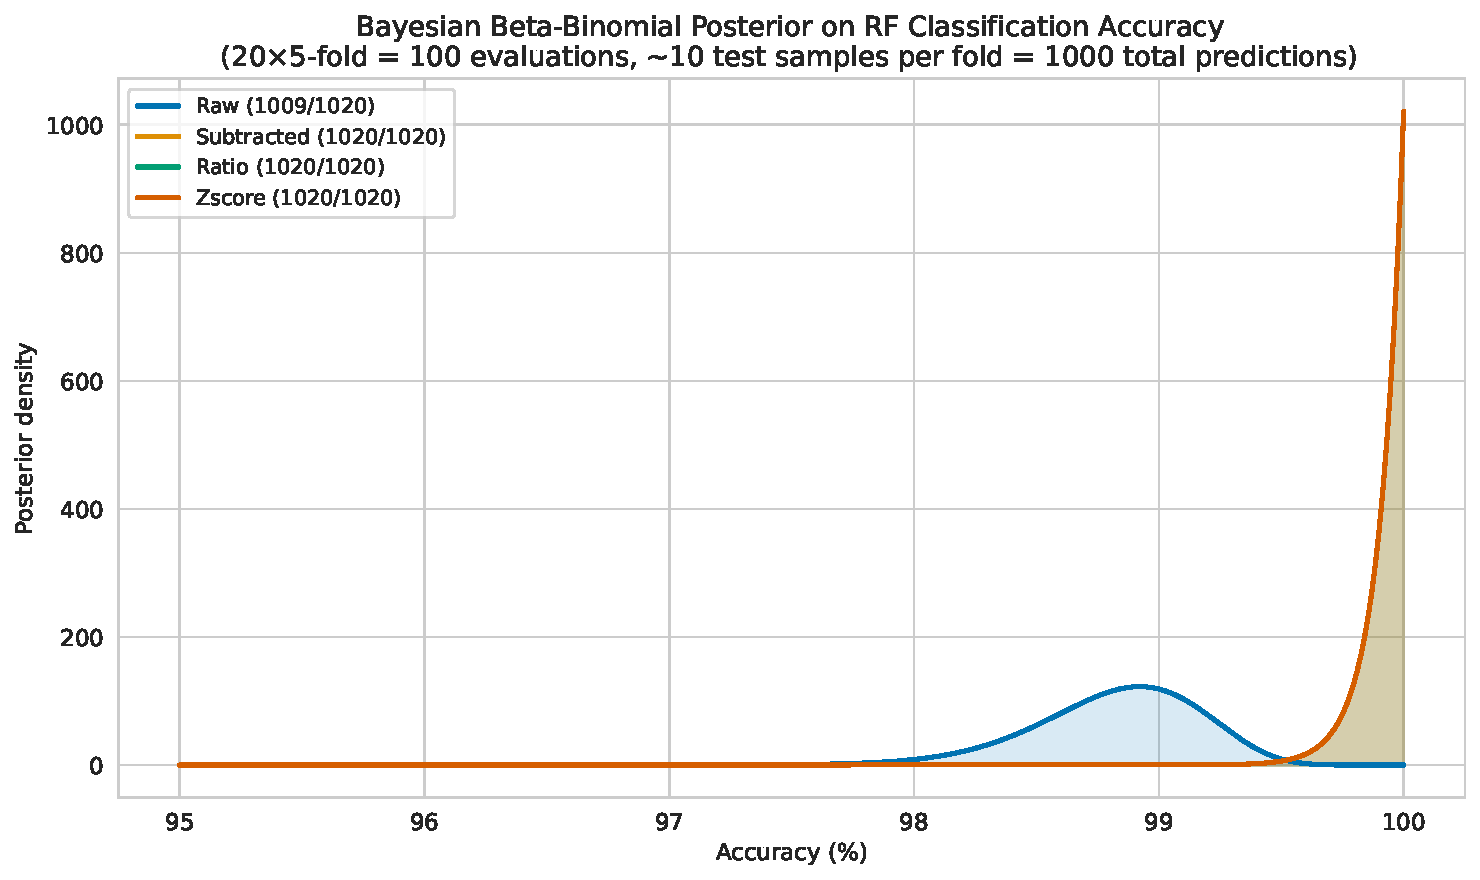
\includegraphics[width=0.75\textwidth]{figures/fig21_bayesian_posterior.pdf}
    \caption{Bayesian Beta-Binomial posterior densities on RF classification accuracy for each isolation method. The raw method's posterior is centered at 98.86\% with non-trivial mass below 99\%, while the three referenced methods concentrate above 99.6\%. The posterior probability that any referenced method exceeds raw is $\geq 0.9997$.}
    \label{fig:bayesian_posterior}
\end{figure}

The posterior accuracy difference between any referenced method and raw has median $1.05\%$ with a 95\% credible interval of $[0.46\%, 1.84\%]$, and $P(\text{referenced} > \text{raw}) \geq 0.9997$. This Bayesian framing provides three advantages over the frequentist tests: (1)~it produces a properly bounded credible interval despite the ceiling effect in the referenced methods, replacing the degenerate frequentist CI $[1.000, 1.000]$ with the principled $[0.9964, 0.99997]$; (2)~it gives a direct probability statement about the comparison rather than a $p$-value against a null hypothesis; and (3)~it makes explicit that the magnitude of the effect, while small in absolute terms ($\sim$1 percentage point), is overwhelmingly likely to be a real positive effect rather than noise. One caveat applies. The Beta--Binomial model treats the 1{,}020 fold-level predictions as independent Bernoulli trials, but they derive from only 51 runs evaluated $\sim$20 times each (raw's 11 errors trace largely to a single borderline run). The effective sample size is therefore closer to 51 than 1{,}020, so the credible interval and $P(\text{referenced} > \text{raw})$ should be read as optimistic upper bounds on certainty rather than calibrated probabilities; the run-level Cliff's-delta analysis, which localizes the effect to one run, is the more conservative summary.

\subsection{Temporal Fingerprints}\label{sec:fingerprints}

Figure~\ref{fig:fingerprint} shows the per-class temporal fingerprints of the most discriminative position-proxy channel (frame\_r2.Mx) across the 20 temporal bins, with each toolpath type's individual runs and mean~$\pm$~std, in both the raw-active and air-cut-subtracted representations.

\begin{figure}[H]
    \centering
    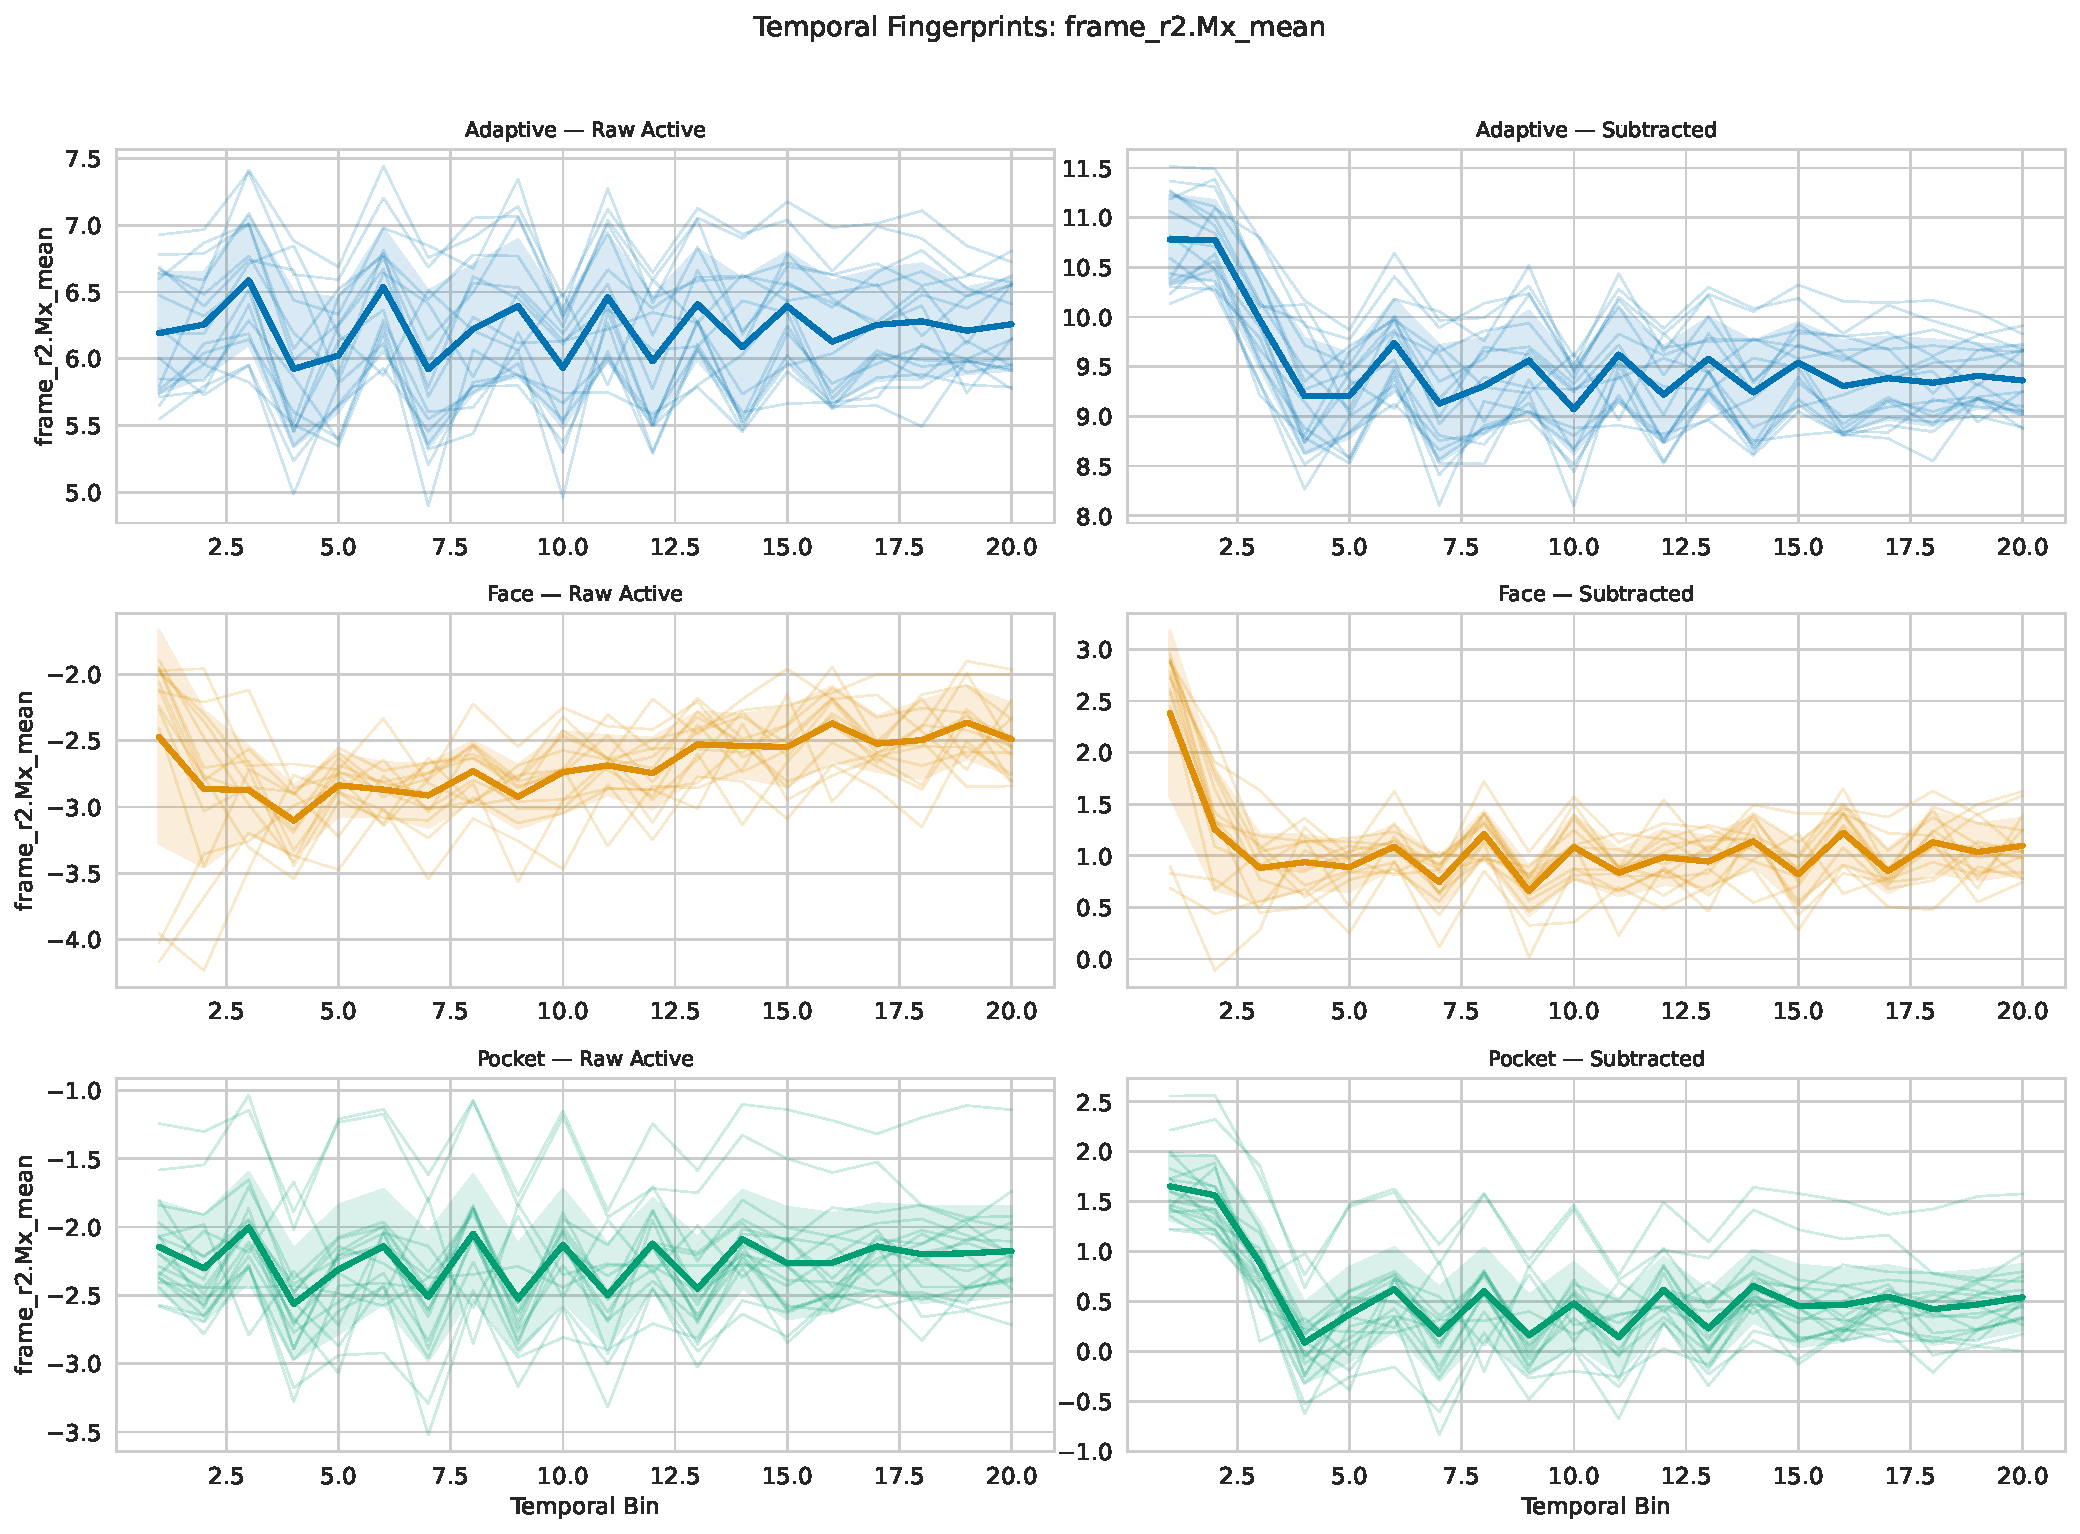
\includegraphics[width=0.9\textwidth]{figures/fig6_temporal_fingerprint.pdf}
    \caption{Temporal fingerprints of the top-ranked position-proxy channel (frame\_r2.Mx mean) across 20 temporal bins, by toolpath type (rows: adaptive, facing, pocketing) and representation (left: raw active; right: air-cut subtracted). Thin lines are individual runs; the bold line and shaded band are the per-type mean~$\pm$~one standard deviation. The three types occupy distinct magnetometer ranges---a workspace-position effect (Section~\ref{sec:physics})---and air-cut subtraction (right column) compresses the inter-type offsets while retaining a residual separation.}
    \label{fig:fingerprint}
\end{figure}

Figure~\ref{fig:fingerprint_overlay} presents the temporal fingerprint overlay, showing how the three toolpath types produce distinct quasi-static sensor signal profiles across normalized program time.

\begin{figure}[H]
    \centering
    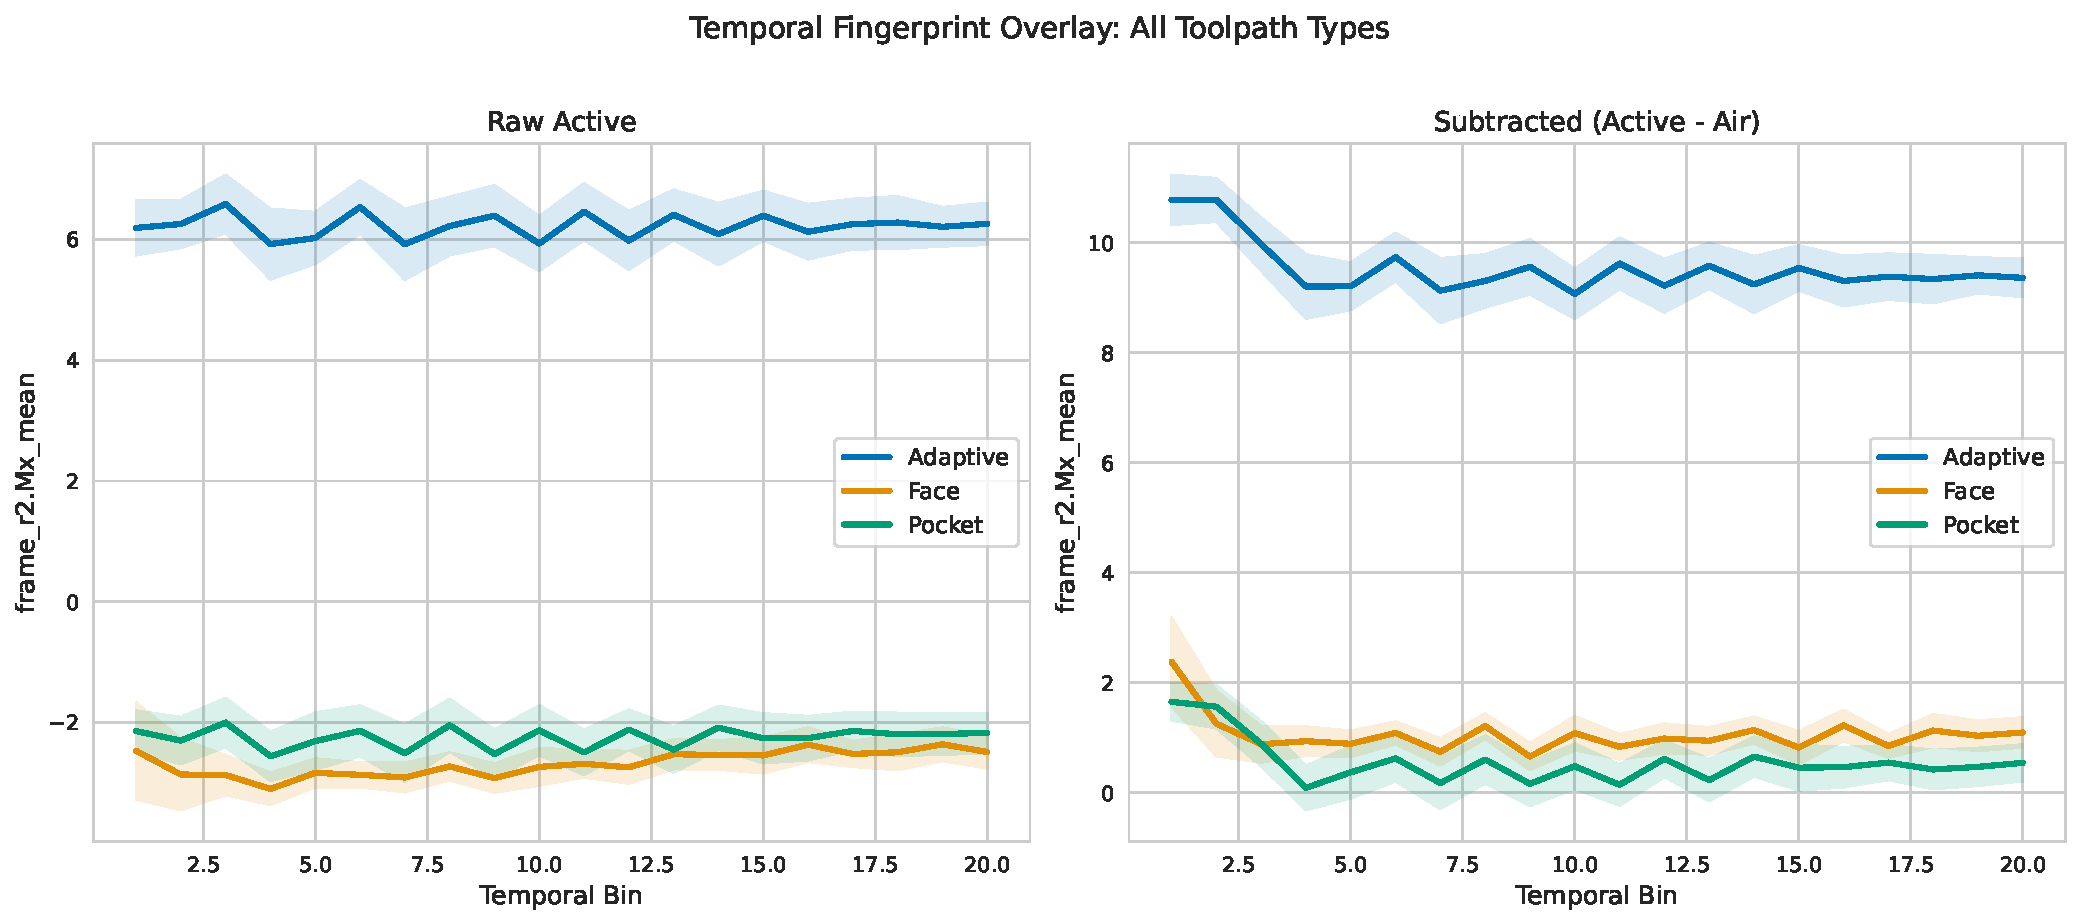
\includegraphics[width=0.85\textwidth]{figures/fig6b_temporal_overlay.pdf}
    \caption{Temporal fingerprint overlay for all three toolpath types. Left: raw active signals. Right: subtracted (air-cut referenced) signals. Shaded regions: $\pm 1$ std. The distinct separation between classes persists after subtraction. Note that these profiles reflect quasi-static motion envelopes rather than cutting vibration dynamics (Section~\ref{sec:sampling}).}
    \label{fig:fingerprint_overlay}
\end{figure}

Adaptive clearing produces the highest absolute magnetometer values (reflecting its workspace location) with gradual temporal variation, while facing and pocketing occupy a different region with more temporal structure. After air-cut subtraction (right panel), the inter-class separation is reduced but still present, confirming that some discriminative information survives the referencing process and is not purely position-dependent.

\subsection{Generalization Analysis}

Table~\ref{tab:generalization} reports leave-$K$-runs-out CV results.

\begin{table}[H]
\caption{Leave-$K$-runs-out accuracy (RF). For $K \geq 2$, results are averaged over 100 random combinations.}\label{tab:generalization}
\centering
\begin{tabular}{lccc}
\toprule
\textbf{Method} & \textbf{$K = 1$} & \textbf{$K = 2$} & \textbf{$K = 3$} \\
\midrule
Raw        & $100.0 \pm 0.0$ & $99.5 \pm 5.0$ & $99.0 \pm 5.7$ \\
Subtracted & $100.0 \pm 0.0$ & $100.0 \pm 0.0$ & $100.0 \pm 0.0$ \\
Ratio      & $100.0 \pm 0.0$ & $100.0 \pm 0.0$ & $100.0 \pm 0.0$ \\
Z-score    & $100.0 \pm 0.0$ & $100.0 \pm 0.0$ & $100.0 \pm 0.0$ \\
\bottomrule
\end{tabular}
\end{table}

Raw features degrade slightly at $K = 3$ (99.0\%), while all referenced methods maintain 100\%, consistent with the repeated CV finding that air-cut referencing improves robustness.

\subsection{Harder Classification Tasks}

To probe the limits of the methodology beyond the easy three-class task, we evaluate several more challenging classification scenarios.

\subsubsection{Six-Class Classification (Toolpath $\times$ Condition)}

Combining the 55 air-cut and 51 active-cut runs into a six-class problem (3 toolpath types $\times$ 2 cutting conditions), the RF classifier achieves $99.1\% \pm 1.8\%$ accuracy. This demonstrates that sensor features can simultaneously distinguish both the toolpath type and the cutting condition (air vs.\ active), with near-perfect separability.

\subsubsection{Air vs.\ Active Discrimination}

Binary classification of air-cut vs.\ active-cut runs (ignoring toolpath type) achieves $99.0\% \pm 1.9\%$ accuracy, confirming that material engagement produces a detectable change in sensor signatures across all toolpath types. Per-toolpath binary discrimination (air vs.\ active within each type) achieves 100\% for all three types.

\subsubsection{Cross-Condition Transfer}

Whether models transfer across cutting conditions is a direct test of the air-cut referencing hypothesis. We train an RF classifier on \textit{air-cut data only} (55 runs, 3 toolpath classes) and test on \textit{active-cut data} (51 runs):

\begin{table}[H]
\caption{Cross-condition transfer accuracy. Models trained on one condition are tested on the other without retraining.}\label{tab:cross_condition}
\centering
\begin{tabular}{lcc}
\toprule
\textbf{Transfer Direction} & \textbf{Accuracy (\%)} & \textbf{Train / Test} \\
\midrule
Air $\rightarrow$ Active   & 37.3 & 55 / 51 \\
Active $\rightarrow$ Air   & 40.0 & 51 / 55 \\
\bottomrule
\end{tabular}
\end{table}

Both transfer directions achieve near-chance accuracy ($\sim$37--40\% vs.\ 33\% random baseline), demonstrating that raw sensor features learned from one cutting condition do not transfer to the other. This result has two implications: (1)~it confirms that the air and active sensor signals are fundamentally different, with the machine dynamics (captured by air cuts) and process dynamics (added by active cuts) producing distinct feature distributions; and (2)~it motivates the air-cut referencing methodology, since the process component isolated by subtraction/normalization may be more transferable than the raw signal.

\subsubsection{Leave-One-Type-Out: Unknown Toolpath Detection}

We train a binary classifier on two toolpath types and examine its behavior when presented with the unseen third type. Since the held-out class was not in the training data, the classifier must assign it to one of the known classes.

\begin{table}[H]
\caption{Leave-one-type-out analysis. An RF classifier trained on two toolpath types is applied to the unseen third type. ``Predicted as'' shows how the unknown type is classified; ``Confidence'' reports the RF posterior probability.}\label{tab:loto}
\centering
\begin{tabular}{llcc}
\toprule
\textbf{Held Out} & \textbf{Predicted As} & \textbf{Mean Conf.} & \textbf{Min Conf.} \\
\midrule
Adaptive (17)  & Pocket: 17/17    & $0.77 \pm 0.05$ & 0.67 \\
Face (15)      & Pocket: 15/15    & $0.79 \pm 0.04$ & 0.71 \\
Pocket (19)    & Adaptive: 16, Face: 3   & $0.63 \pm 0.06$ & 0.52 \\
\bottomrule
\end{tabular}
\end{table}

When adaptive or face toolpaths are held out, the classifier consistently predicts ``pocket'' with moderate confidence (0.67--0.79). When pocket is held out, predictions split between adaptive (84\%) and face (16\%) with lower confidence (min 0.52). The reduced confidence for unknown types suggests that a confidence-thresholding approach could potentially detect novel toolpath types, a direction for future work in anomaly detection.
